\documentclass[11pt, oneside]{article} 
\usepackage{geometry}                		
\geometry{letterpaper}                   		
\usepackage{graphicx}
\usepackage{graphics}
\usepackage{hyperref}
\usepackage{fancybox}
\usepackage[centertags]{amsmath}
\usepackage{amssymb}
\usepackage{amsthm}			
\usepackage{natbib}				
\usepackage{fullpage}
\usepackage{placeins}
\usepackage{setspace}
\usepackage{lineno}
%\usepackage{figcaps}
\usepackage[tablesfirst,nolists]{endfloat}
\usepackage{authblk}
\usepackage{csvsimple}


\DeclareRobustCommand{\firstsecond}[2]{#1}

\newcommand{\mb}{\mathbf}
\newcommand{\bs}{\boldsymbol}
\newcommand{\wt}{\widetilde}
\newcommand{\s}{^{(s)}}

\title{Supplemental Methods}

\author[1]{}
\author[2]{}
\author[3]{}

\date{\today}

\begin{document}
\maketitle

\doublespacing

\section {Data overview}
This document briefly describes the data cleaning, subsetting, and aggregation methods specific to each dataset.
%Table \ref{metadata} shows metadata on the datasets included in the meta-analysis.
We plot species accumulation curves, spatio-temporal variation in the number of taxa observed, the spatio-temporal sampling effort, and the number of taxa shared by each pairwise combination of plots within the study.
%We also identify any potential issues with the data.
We visually evaluated the species accumulation curves and temporal patterns in species abundances. % to screen for changes in sampling methods or data recording methods over the course of the study that could affect results.
A sudden jump in the cumulative number of taxa, for example, could indicate that taxa were recorded to a finer resolution (not that more taxa appeared  at the site).  
A species accumulation curve that does not level off could indicate a community undergoing rapid succession, invasion, or environmental change. 

For each dataset, we evaluated whether all sites were observed with equal effort in all years of study and we document any years, sites, sampling occasions,  or species that were droppped from the dataset prior to analysis. 
We also document the method used to aggregate the data to an annual value for each species at each site.
We visually evaluated the species accumulation curves and temporal patters in species abundances to screen for changes in sampling methods or data recording methods over the course of the study that could affect results.
For example, a sudden jump in the number of taxa in a given year could indicate that taxa were recorded to a finer resolution (not that more taxa were actually present at the site).  
We also checked to be sure an abundance of zero was recorded for each absence (i.e. we made sure zeros were filled in for site-years in which a species was not observed).
We removed species codes that obviously represent`unknown' species.
{\bf Do we use cutoff criteria to remove rare species prior to analysis? 
If so, we  should probably include that code in formatting script for each site so that the Supplemental figures and L3 data product we publish match the data used in analysis.}
We also include a table of datasets that were considered, and that we prepared into the L3 format, but ultimately were not included in the analysis (Table \ref{not_used}).


\begin{table}[h!]
\scriptsize
   \centering
     \caption{Metadata on the data sets included in the meta-analysis. This table is automatically generated directly from the datasets in the L3 folder. I can make it look prettier once it is final.} 

\csvautotabular{metadata_table.csv}
   \label{metadata} 
\end{table}


\begin{table}[h!]
\scriptsize
   \centering
     \caption{This is a record of the datasets we considered using and created an L3 dataset for, but did not make the final cut for one reason or another.} 
   \begin{tabular}{lc} 
\\
\hline 
\hline
Dataset &Reason excluded\\
\hline
mcm-diatoms & highly irregular sampling\\
ntl-macroinvertebrates & only four taxa\\
   \end{tabular}

   \label{not_used} 
\end{table}


%%%%%%%%%%%%%%%%%%%%%
\section {Marine datasets}


\subsection {csun.usvi-coral}
Data are from Max Castorani.
Need more metadata for this dataset.
Margaret is looking for data API.
Data are in Figure \ref{usvi-coral}.

\begin{figure}[h!]
\centering
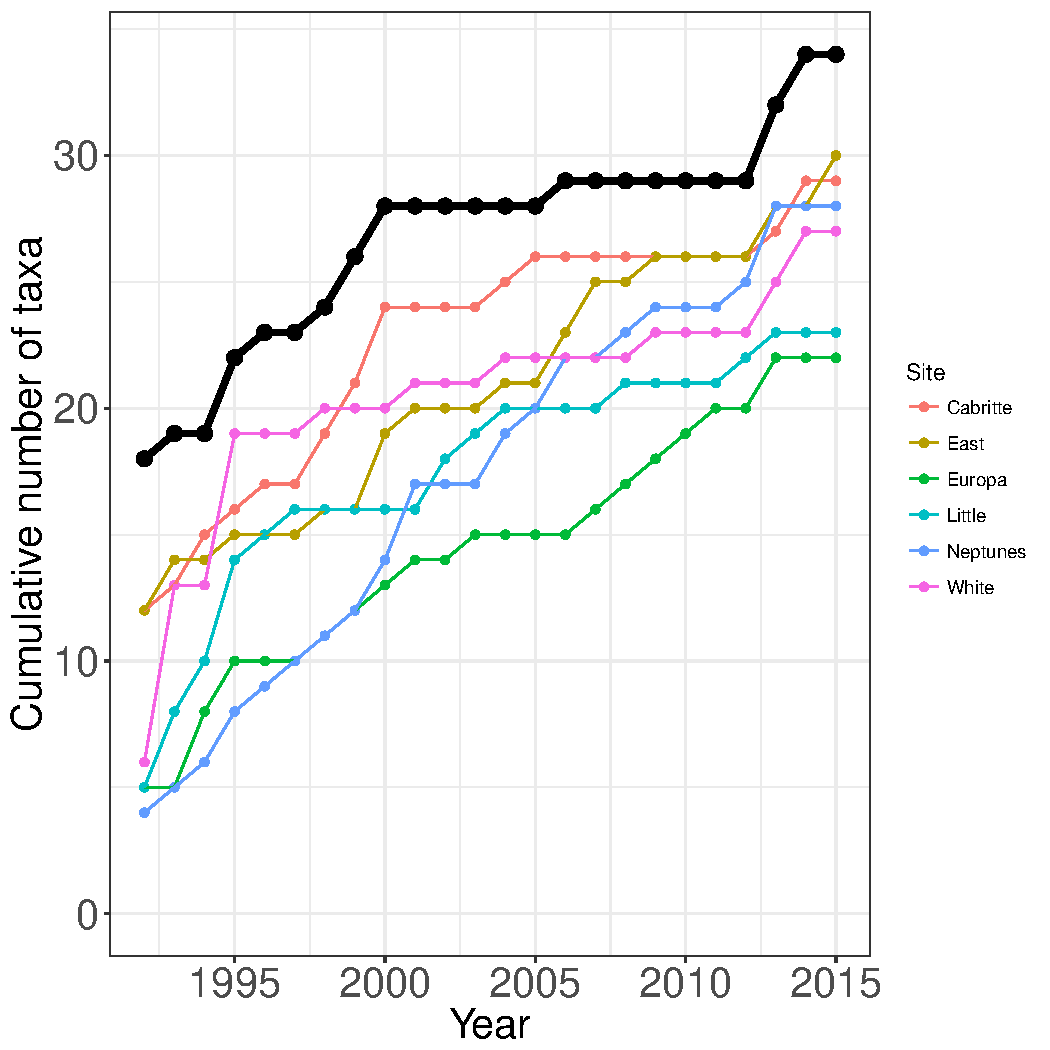
\includegraphics[scale = 0.4]{usvi-coral-castorani_species_accumulation_curve.pdf}
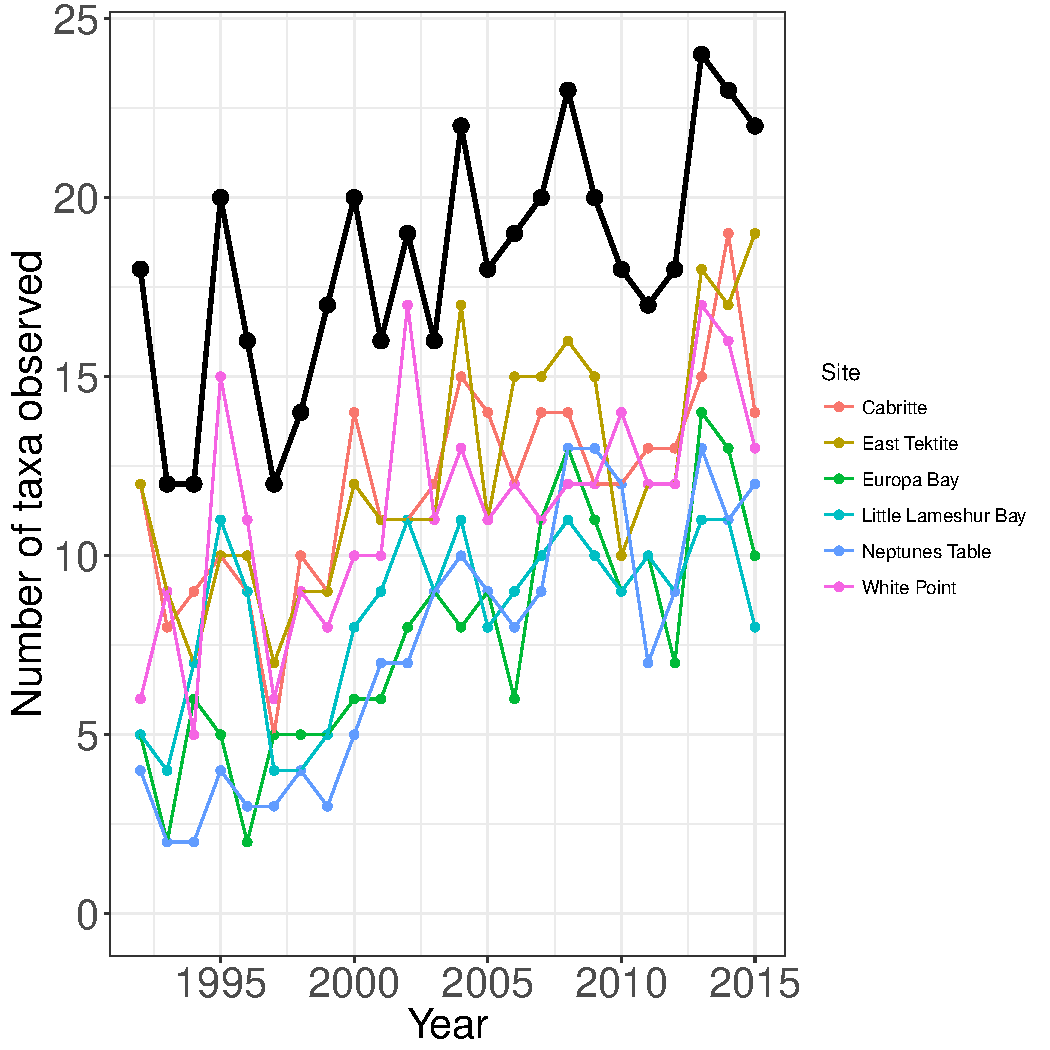
\includegraphics[scale = 0.4]{usvi-coral-castorani_num_taxa_over_time.pdf}
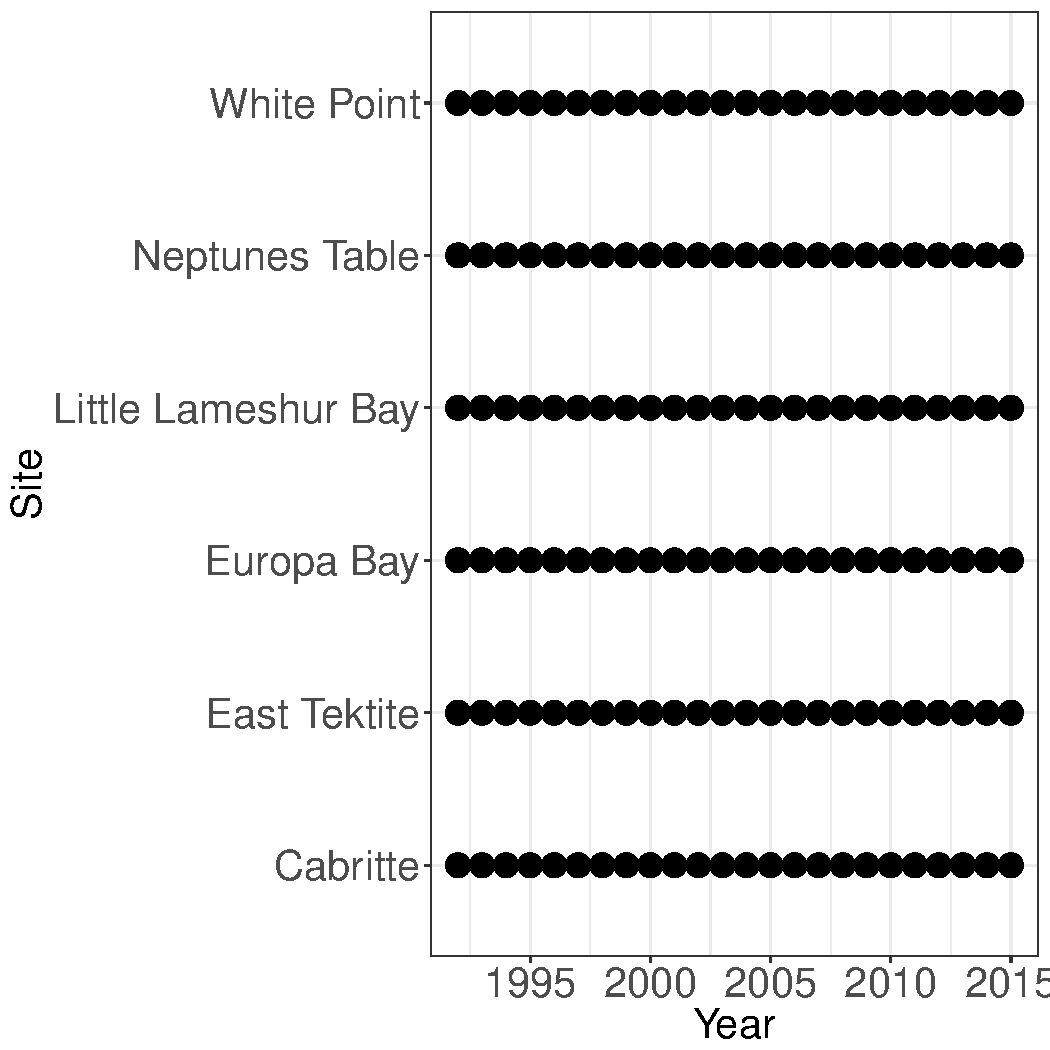
\includegraphics[scale = 0.4]{usvi-coral-castorani_spatiotemporal_sampling_effort.pdf}
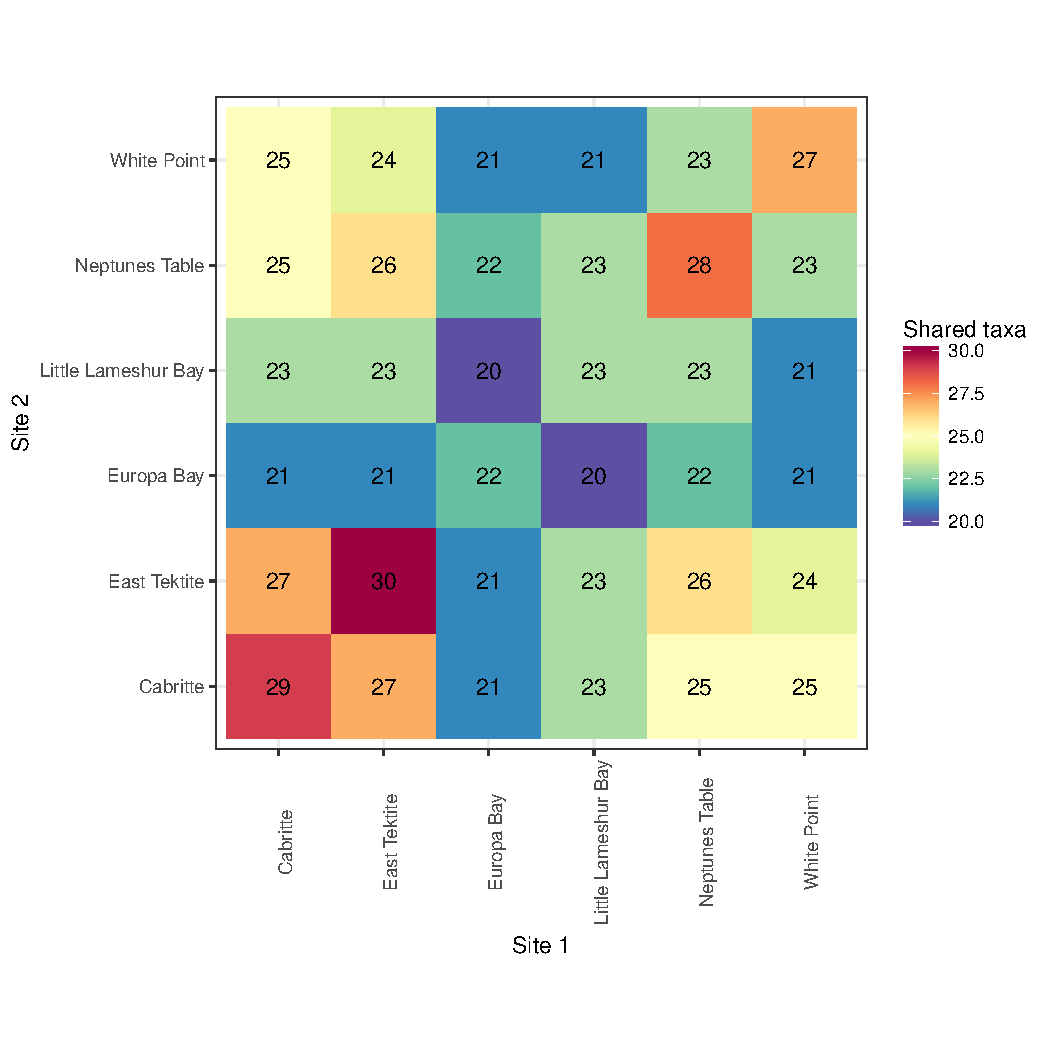
\includegraphics[scale = 0.4]{usvi-coral-castorani_spp_shared.pdf}
\caption{{\bf USVI-corals:} Species accumulation curves (top left),  annual richness (top right), sampling effort (bottom left), and number of shared species (bottom right)  for 34 coral taxa observed at 6 plots on St. John, US Virgin Islands (1990-2005). The black lines represent total site-level values across all plots.}
\label{usvi-coral}
\end{figure}

\subsection {sbc-survey-algae}
{\bf Waiting for updated data to be archived on EDI.}
Two of the eleven sites were initiated in the third year of study.
I think we should remove the two sites.
Data are shown in Figure \ref{sbc-algae}
\begin{figure}[h!]
\centering
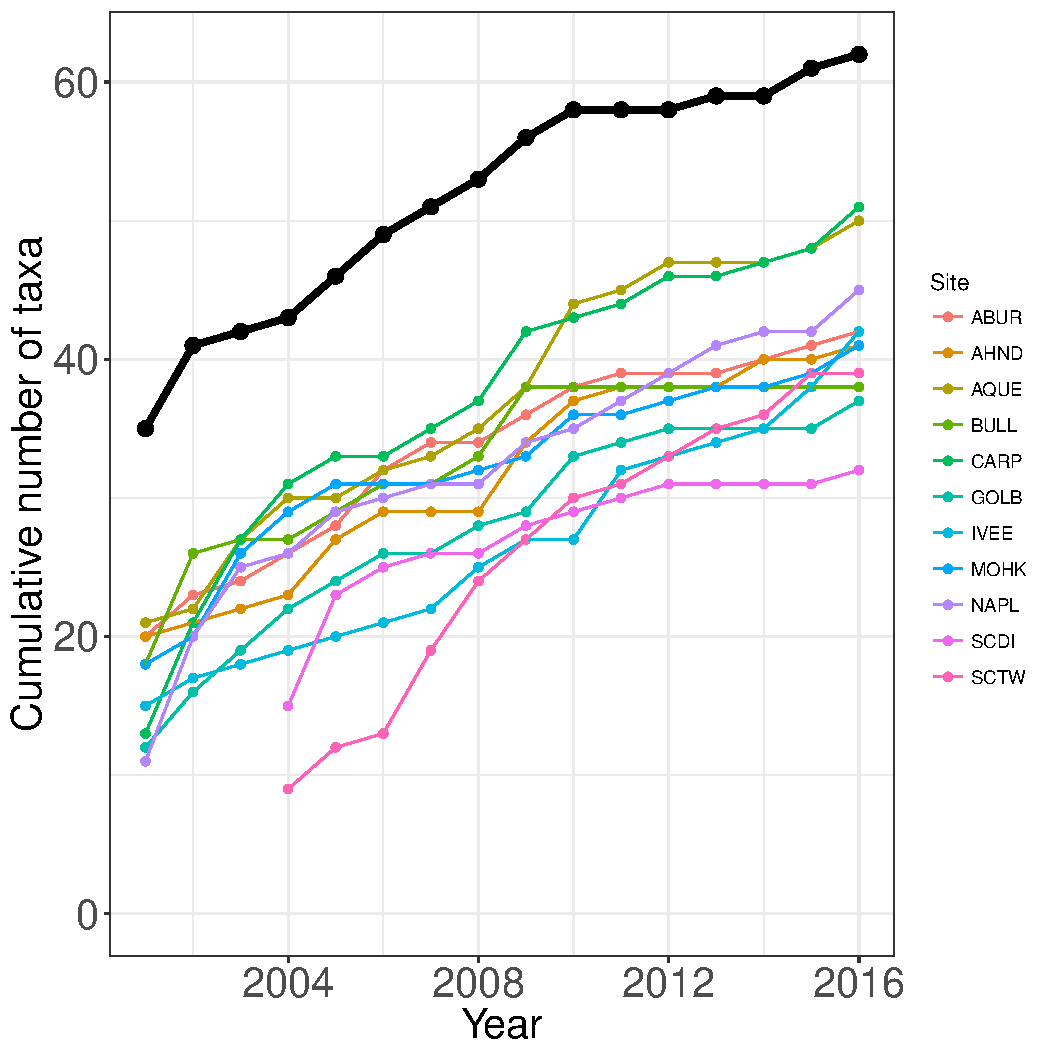
\includegraphics[scale = 0.4]{sbc-algae-castorani_species_accumulation_curve.pdf}
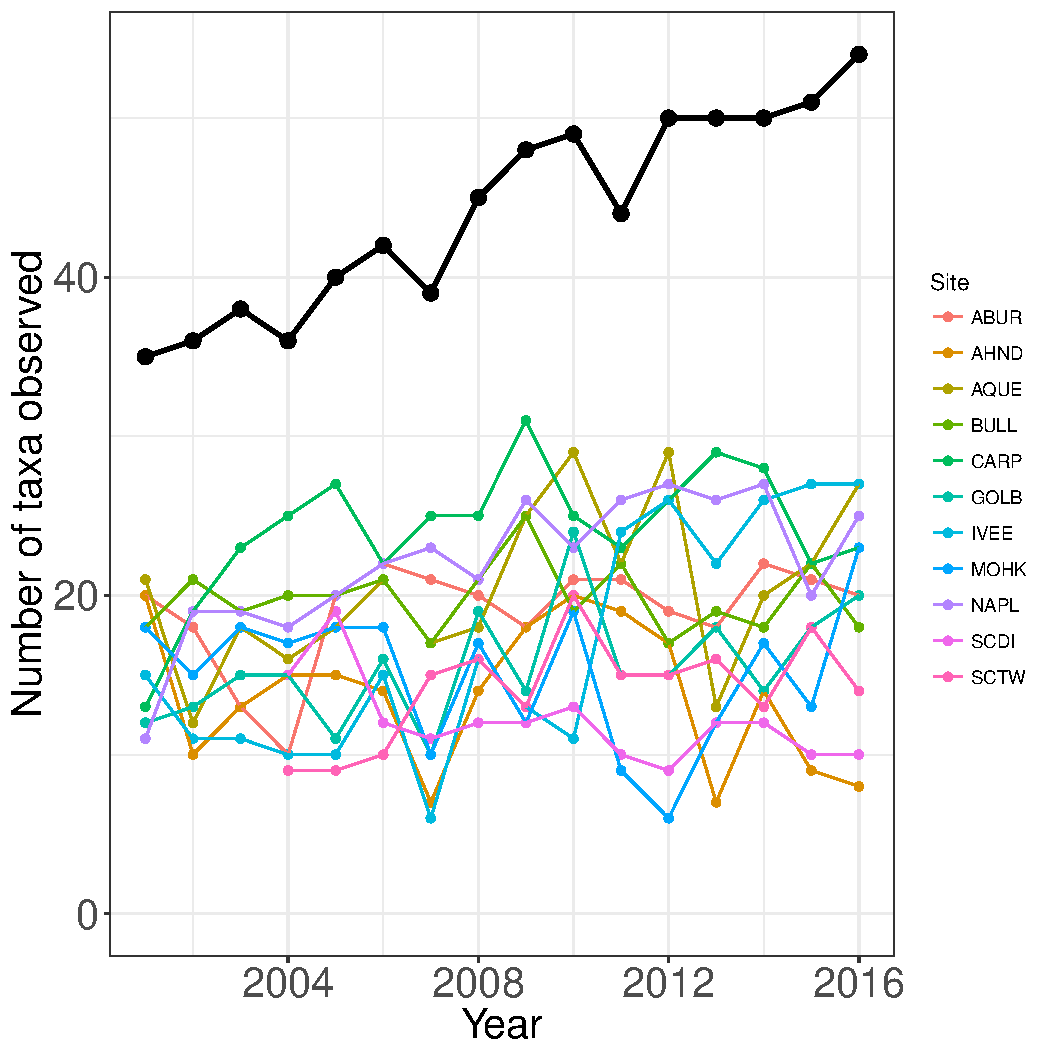
\includegraphics[scale = 0.4]{sbc-algae-castorani_num_taxa_over_time.pdf}
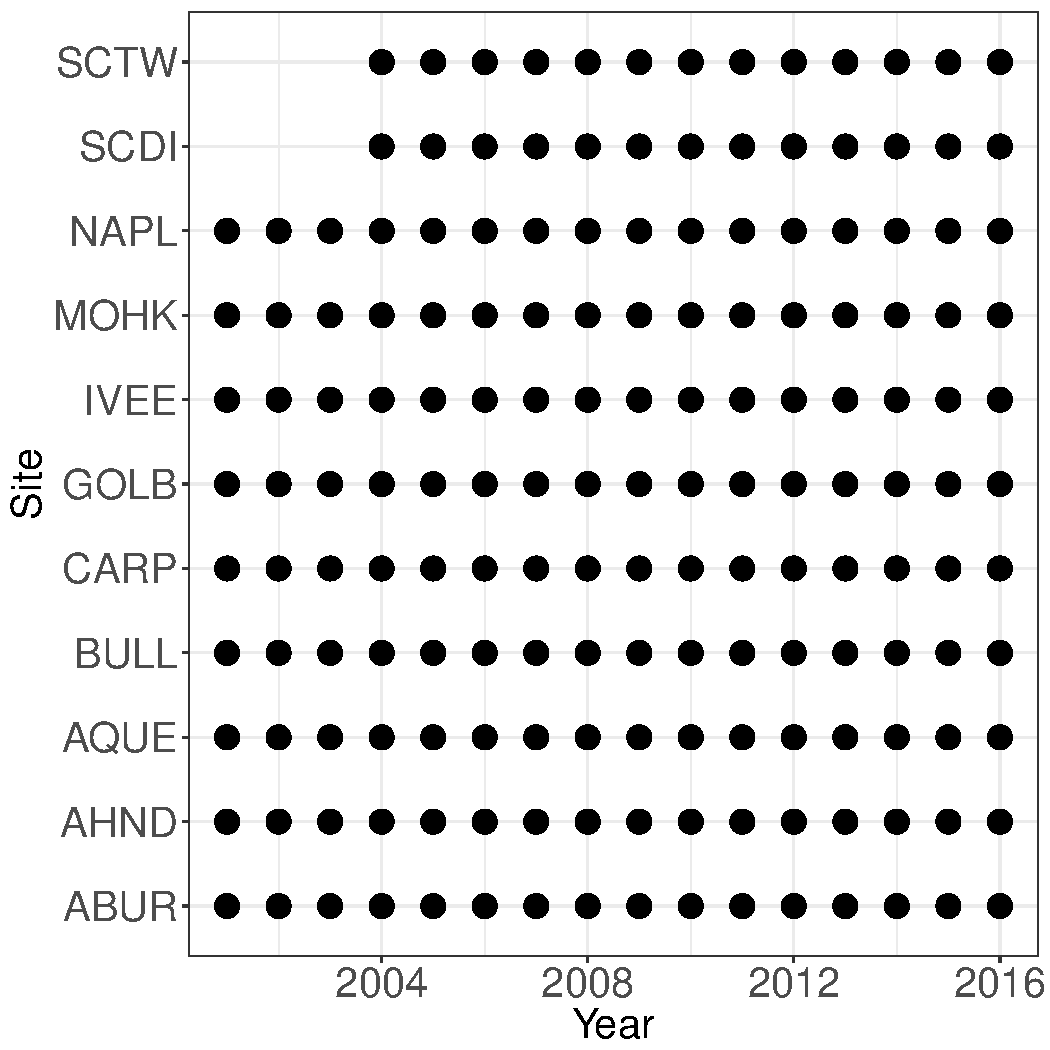
\includegraphics[scale = 0.4]{sbc-algae-castorani_spatiotemporal_sampling_effort.pdf}

\caption{{\bf SBC-algae:} Species accumulation curves (top left),  annual richness (top right), and sampling effort (bottom)  for 62 algae taxa observed at 11 plots in the Santa Barbara Channel LTER (2001-2016). The black lines represent total site-level values across all plots.}
\label{sbc-algae}
\end{figure}

\subsection {sbc-survey-sessile-inverts}
{\bf Waiting for updated data to be archived on EDI.}
Two of the eleven sites were initiated in the third year of study.
I think we should remove the two sites.
Data are shown in Figure \ref{sbc-sessileInverts}
\begin{figure}[h!]
\centering
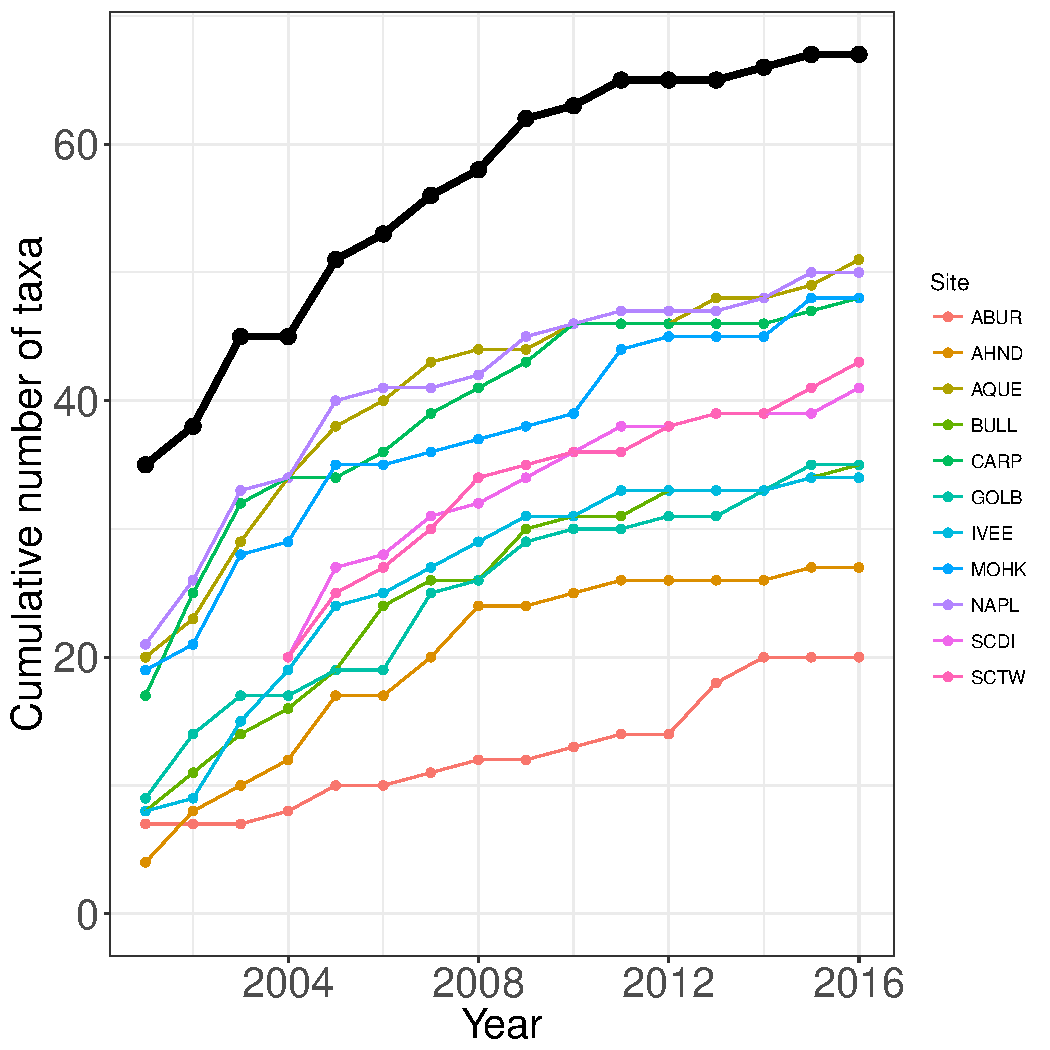
\includegraphics[scale = 0.4]{sbc-sessileInverts-castorani_species_accumulation_curve.pdf}
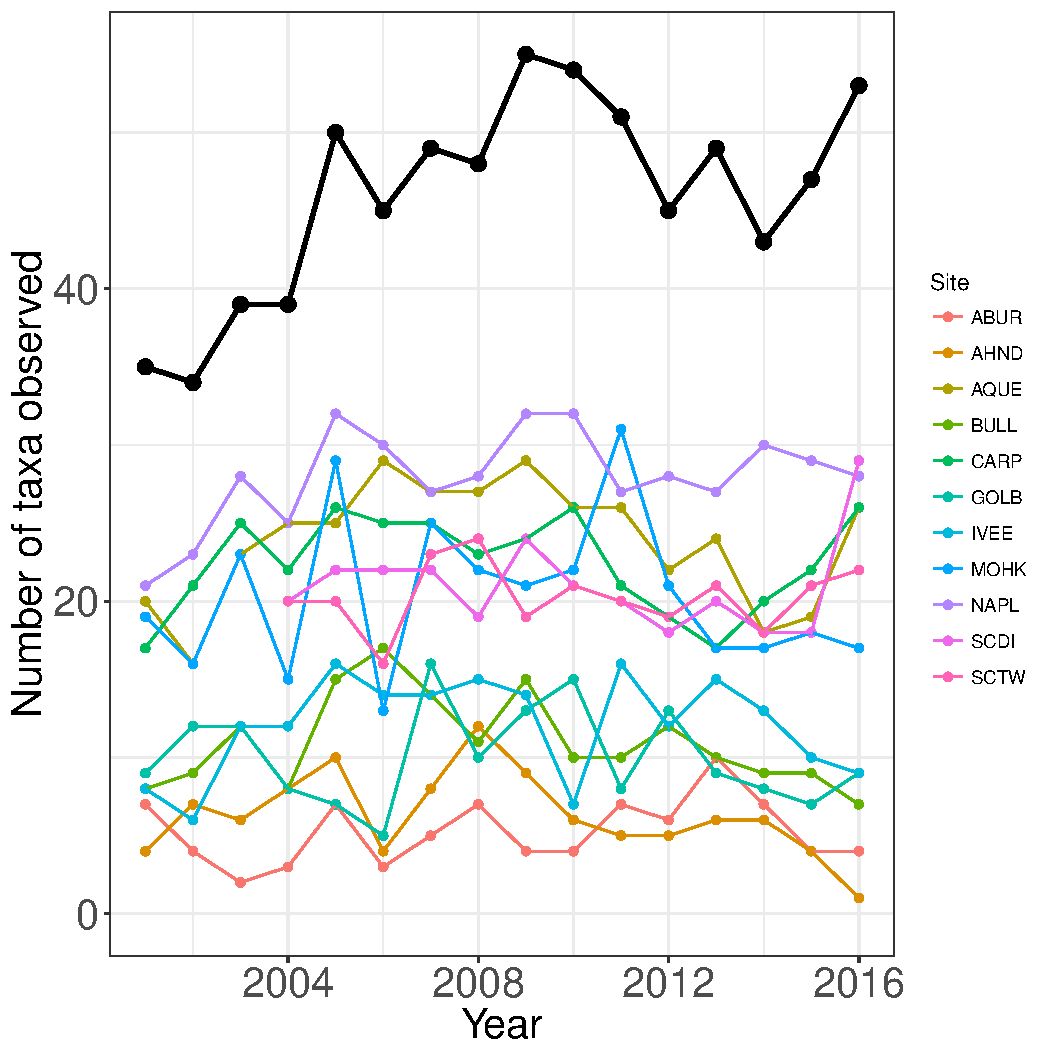
\includegraphics[scale = 0.4]{sbc-sessileInverts-castorani_num_taxa_over_time.pdf}
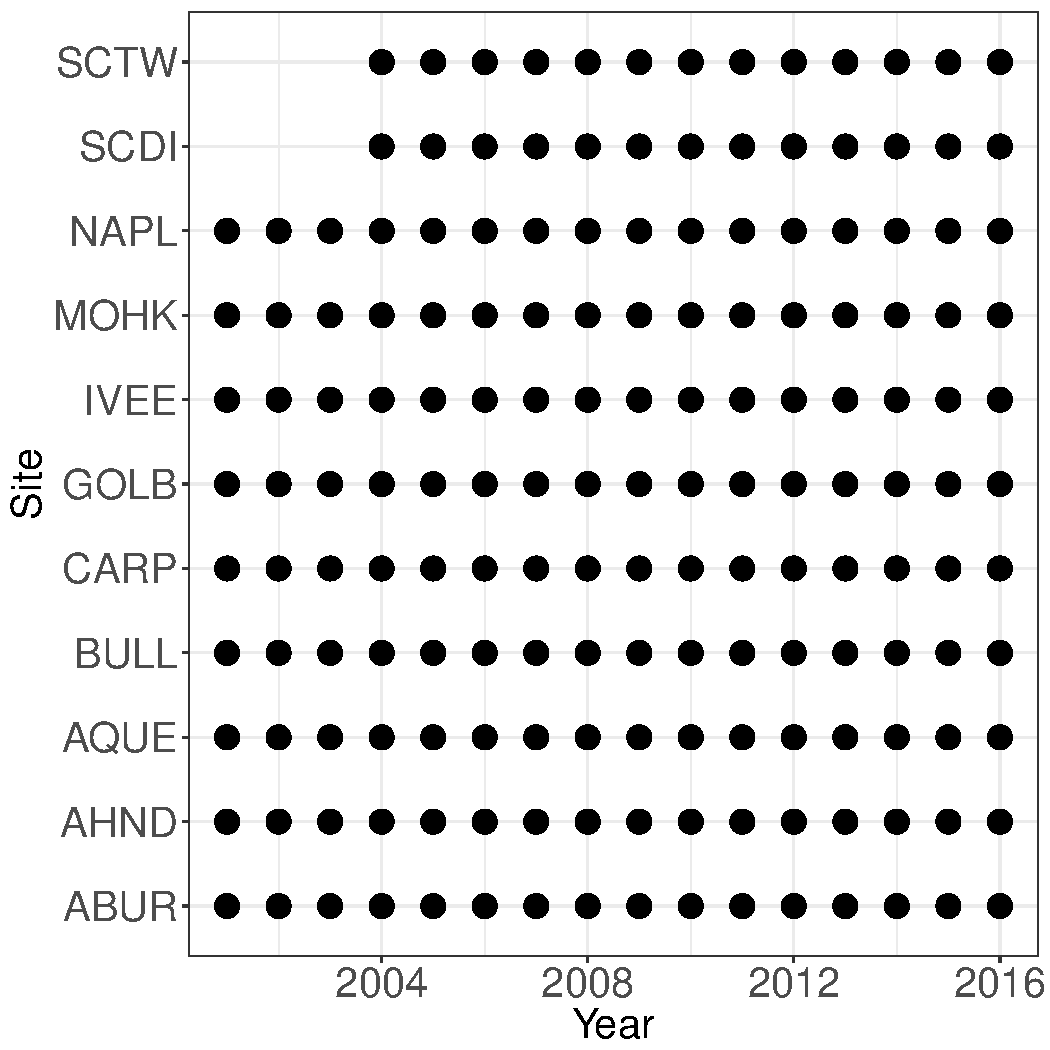
\includegraphics[scale = 0.4]{sbc-sessileInverts-castorani_spatiotemporal_sampling_effort.pdf}
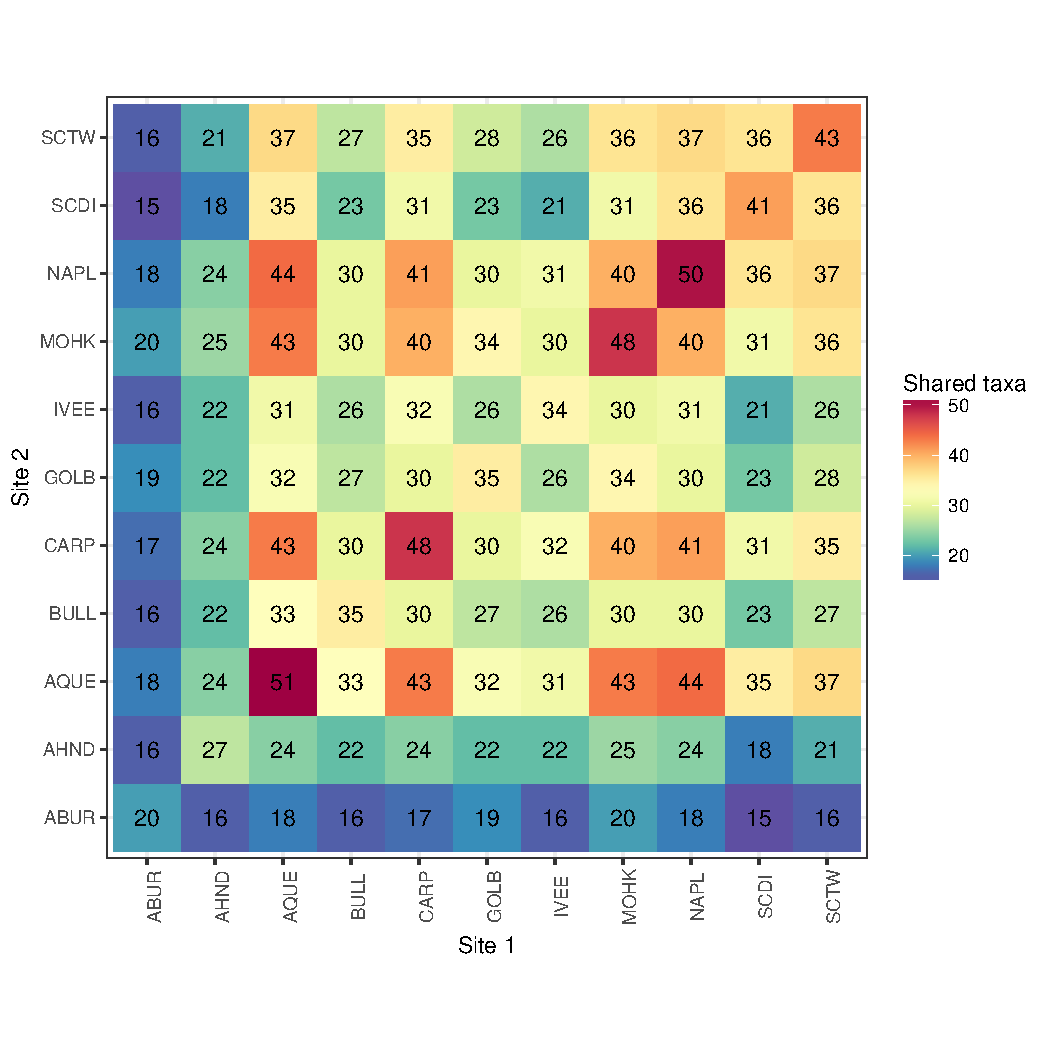
\includegraphics[scale = 0.4]{sbc-sessileInverts-castorani_spp_shared.pdf}
\caption{{\bf SBC-sessile invertebrates:} Species accumulation curves (top left),  annual richness (top right), sampling effort (bottom left), and number of shared species (bottom right)  for 70 sessile invertebrate taxa observed at 11 plots in the Santa Barbara Channel LTER (2001-2016). The black lines represent total site-level values across all plots.}
\label{sbc-sessileInverts}
\end{figure}

\subsection {sbc-survey-mobile-inverts}
{\bf Waiting for updated data to be archived on EDI.}
Two of the eleven sites were initiated in the third year of study.
I think we should remove the two sites.
Data are shown in Figure \ref{sbc-mobileInverts}
\begin{figure}[h!]
\centering
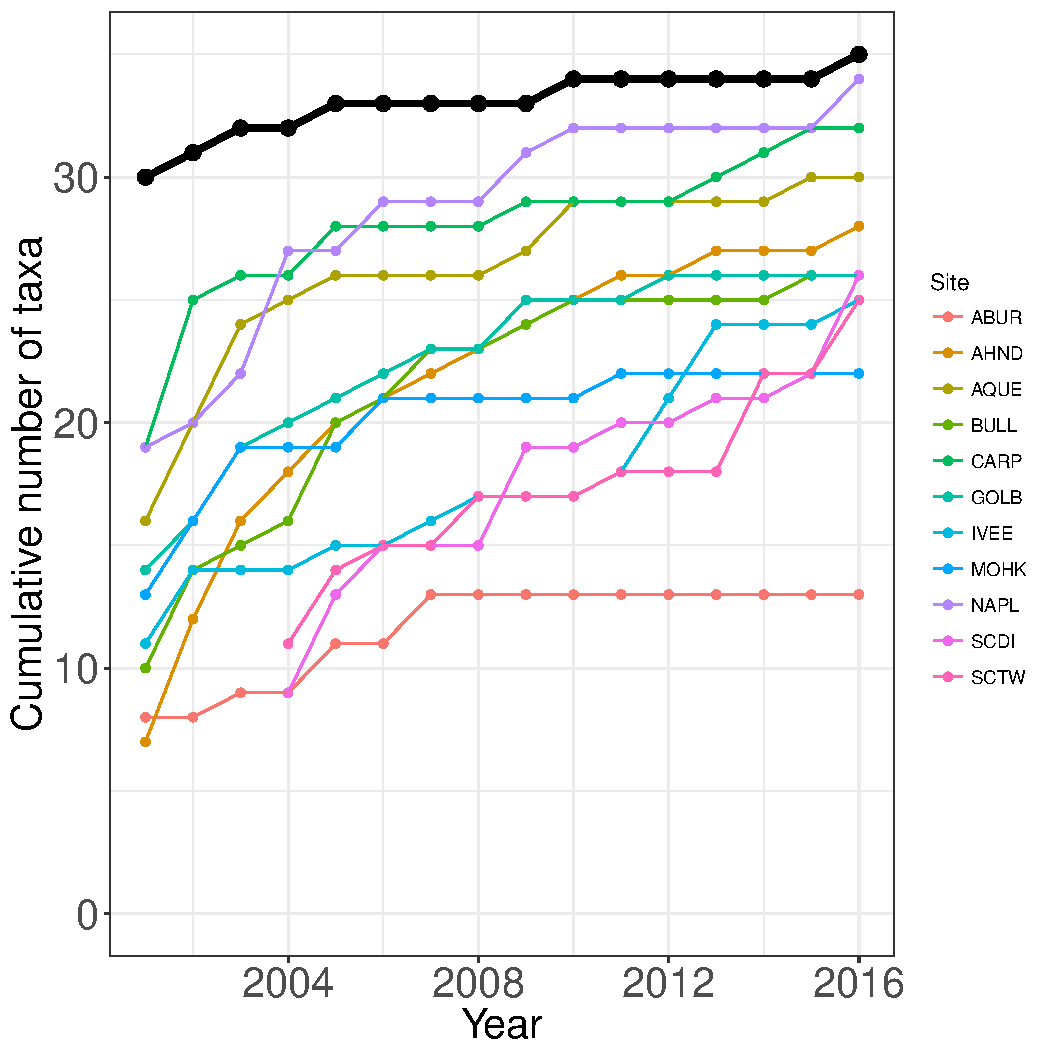
\includegraphics[scale = 0.4]{sbc-mobileInverts-castorani_species_accumulation_curve.pdf}
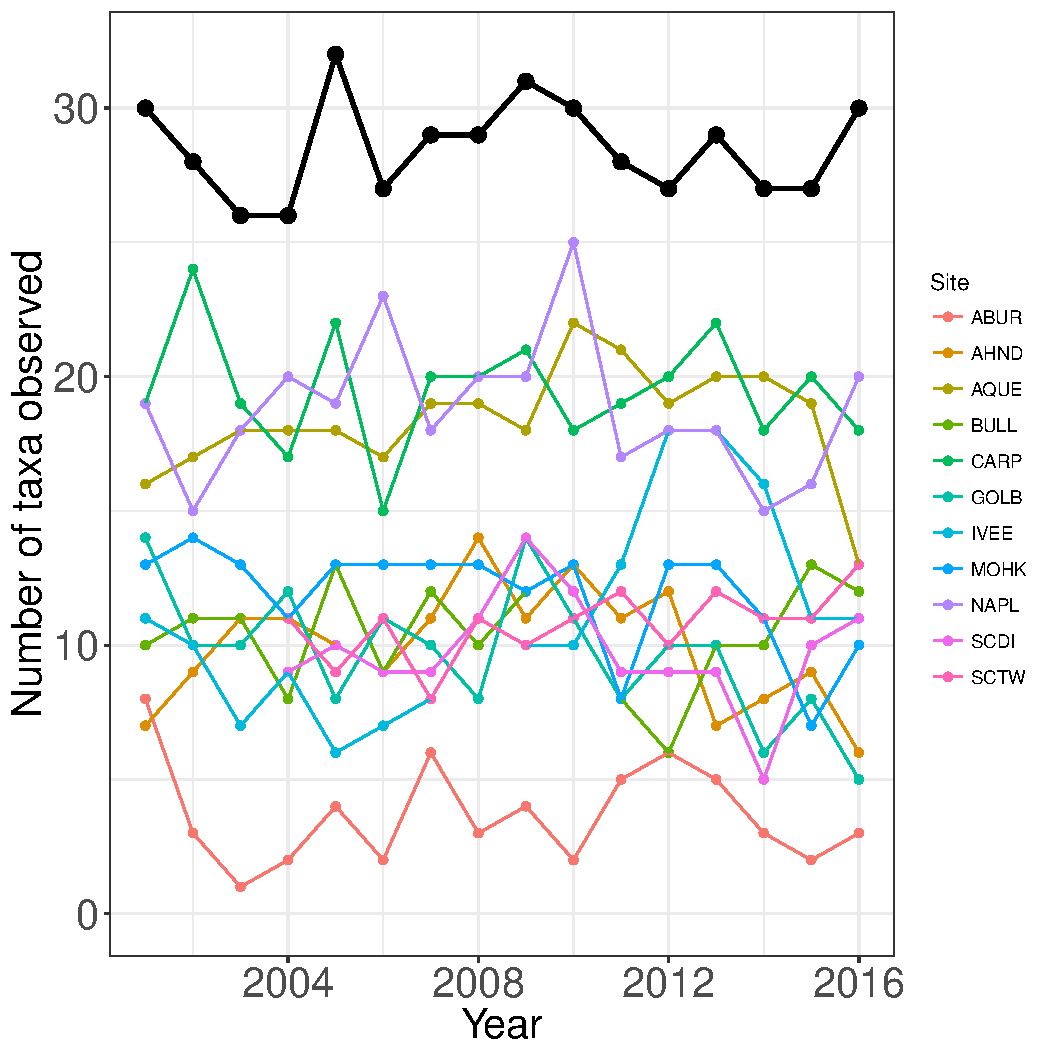
\includegraphics[scale = 0.4]{sbc-mobileInverts-castorani_num_taxa_over_time.pdf}
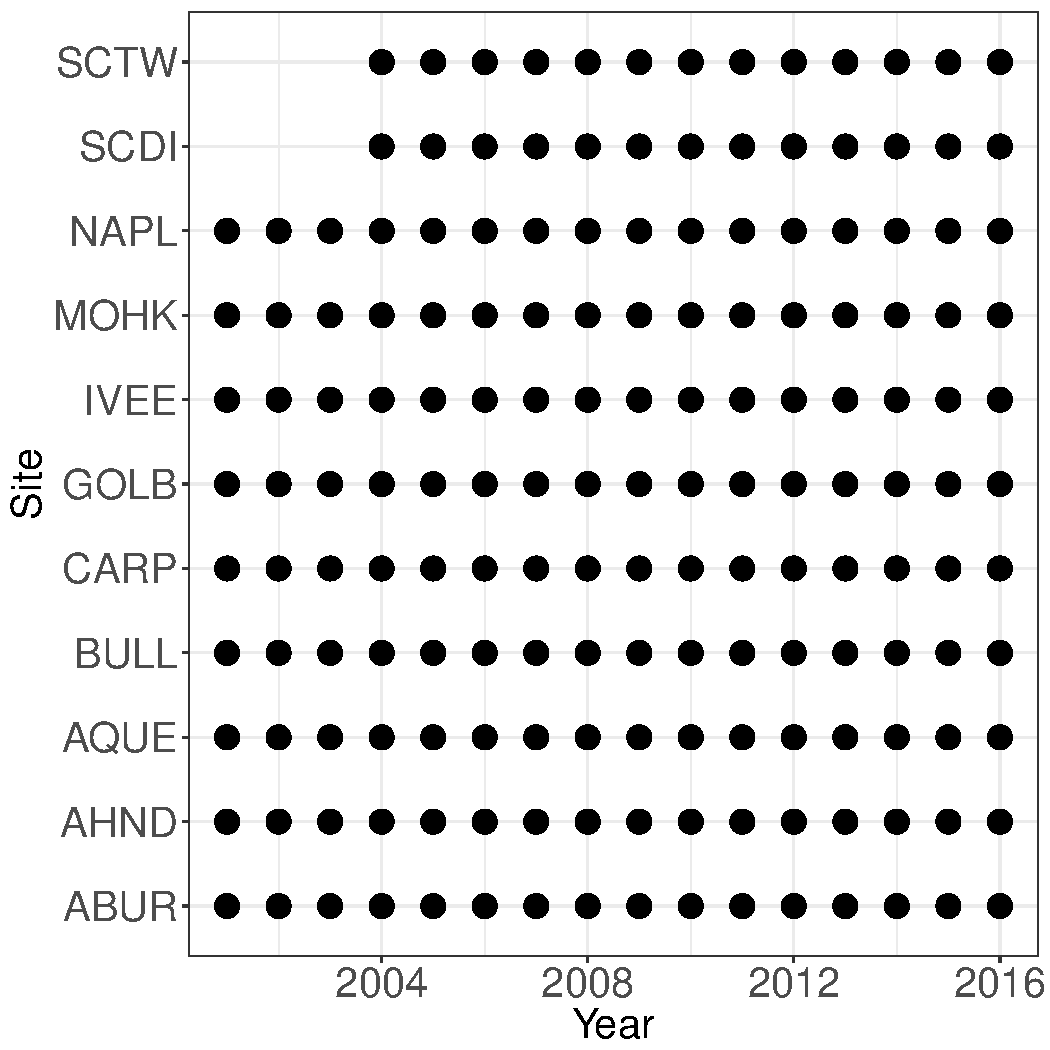
\includegraphics[scale = 0.4]{sbc-mobileInverts-castorani_spatiotemporal_sampling_effort.pdf}
\caption{{\bf SBC-mobile invertebrates:} Species accumulation curves (top left),  annual richness (top right), and sampling effort (bottom)  for 36 mobile invertebrate taxa observed at 11 plots in the Santa Barbara Channel LTER (2001-2016). The black lines represent total site-level values across all plots.}
\label{sbc-mobileInverts} I think we should remove the two sites.
Data are shown in Figure \ref{sbc-fish}
\begin{figure}[h!]
\centering
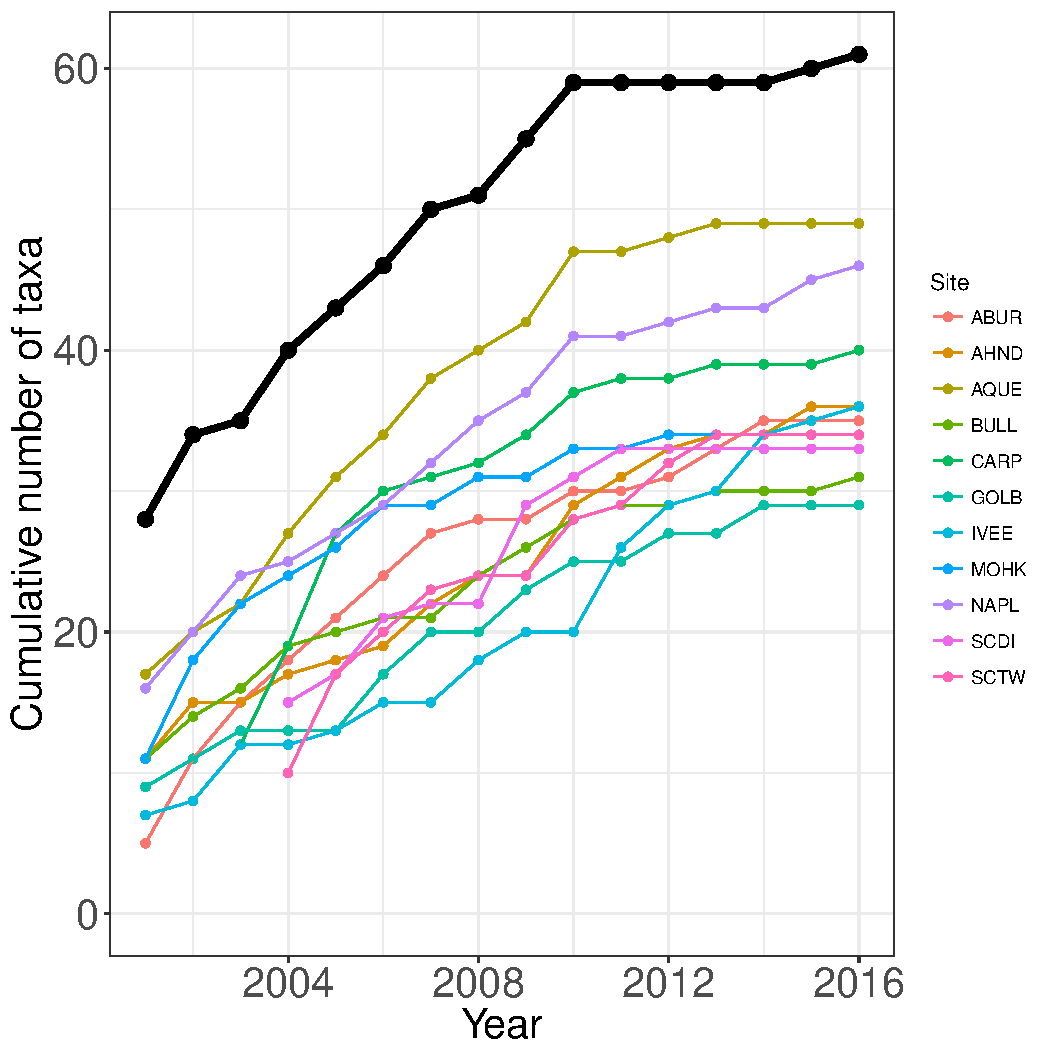
\includegraphics[scale = 0.4]{sbc-fish-castorani_species_accumulation_curve.pdf}
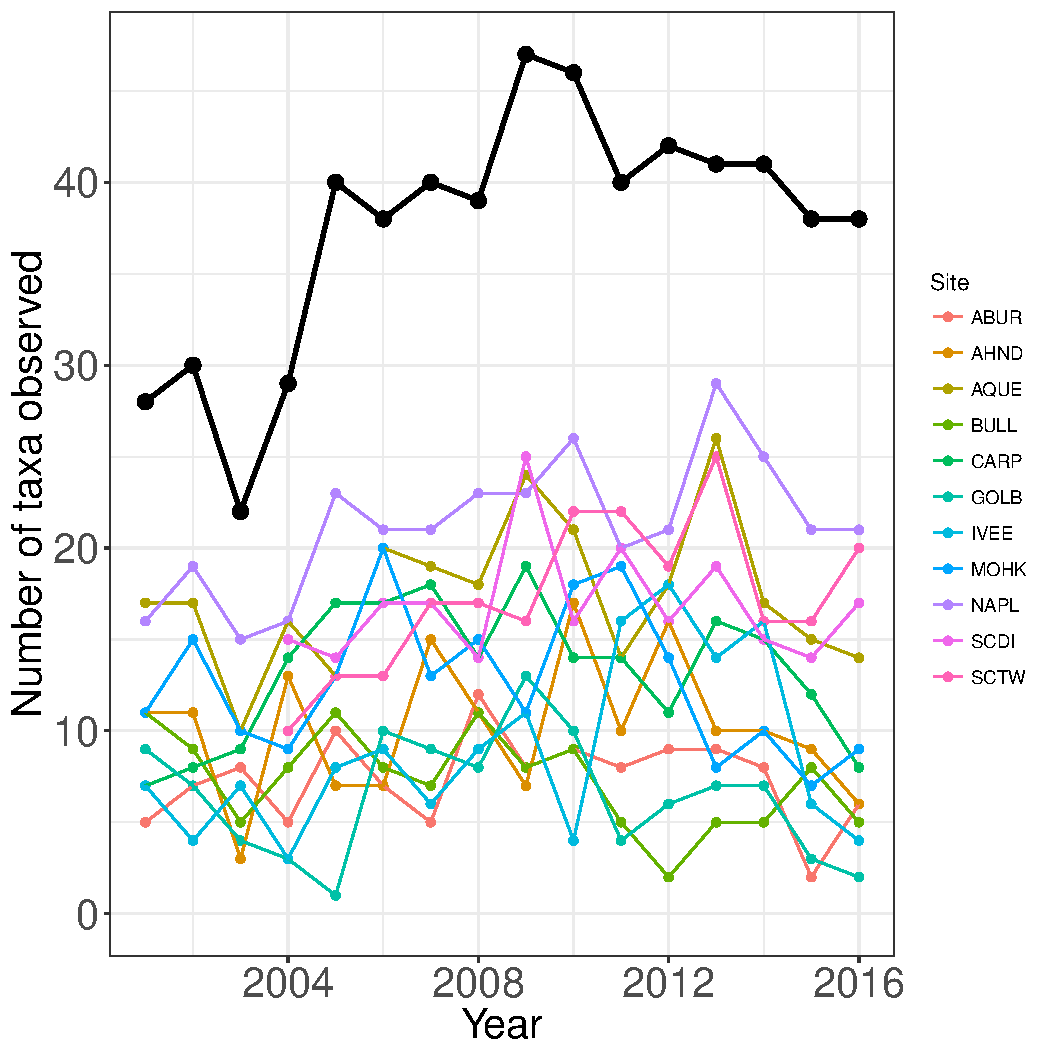
\includegraphics[scale = 0.4]{sbc-fish-castorani_num_taxa_over_time.pdf}
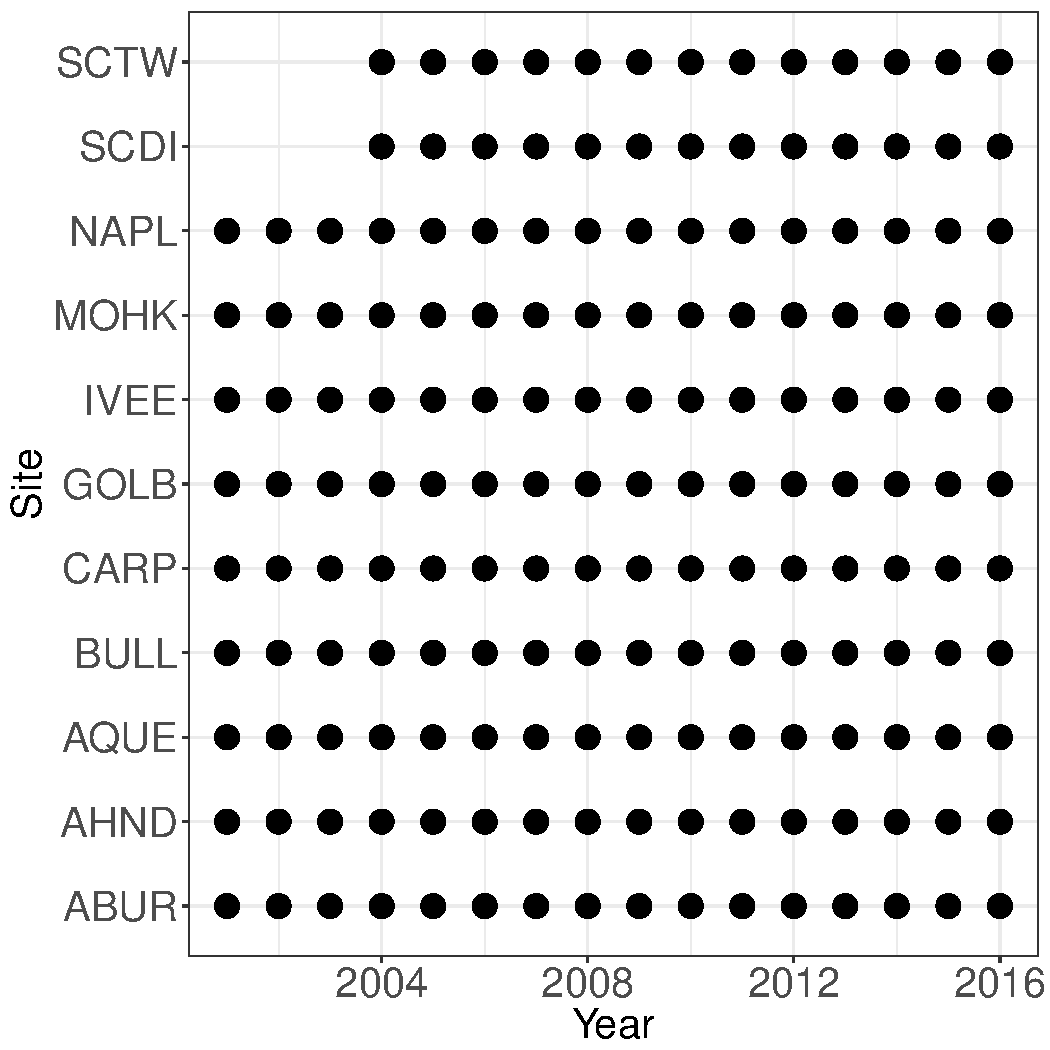
\includegraphics[scale = 0.4]{sbc-fish-castorani_spatiotemporal_sampling_effort.pdf}
%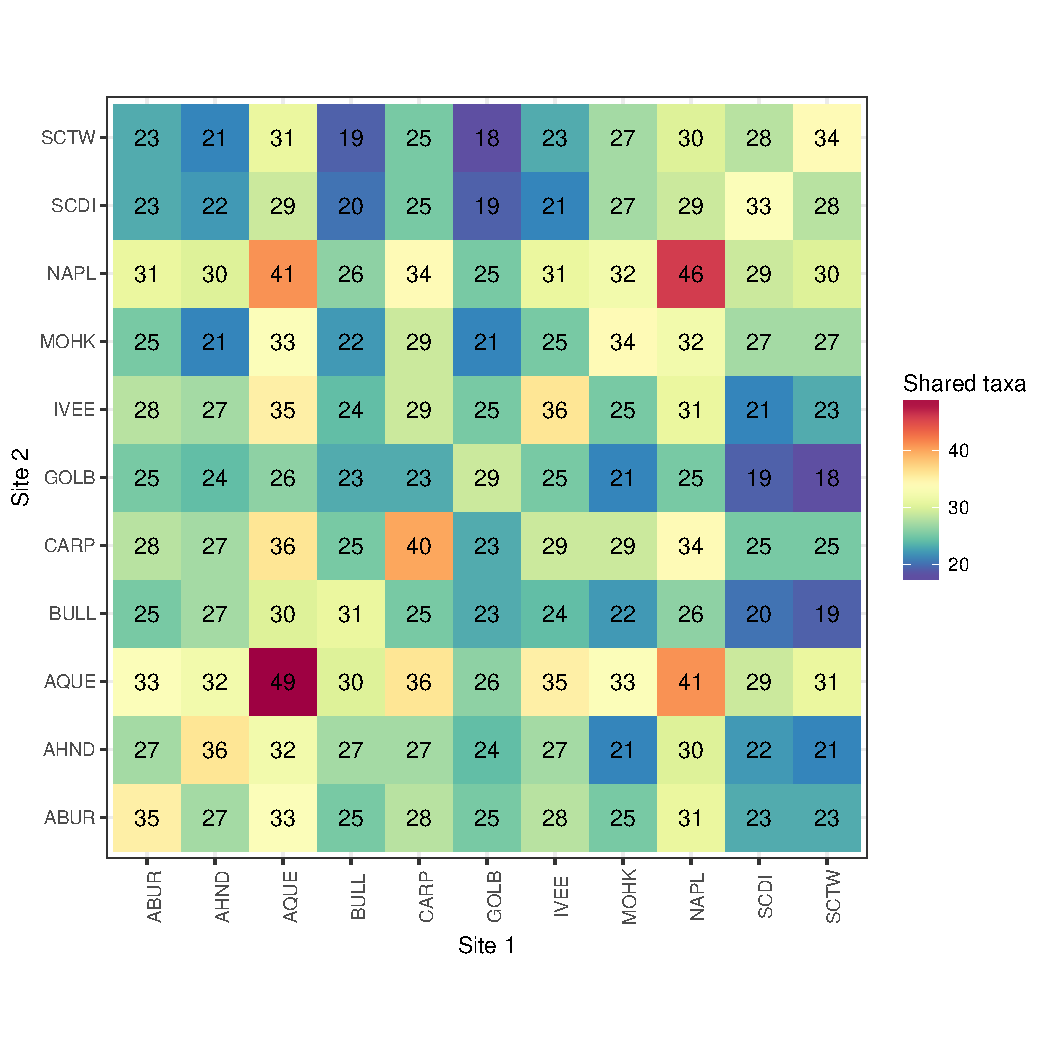
\includegraphics[scale = 0.4]{sbc-fish-castorani_spp_shared.pdf}
\caption{{\bf SBC-fish:} Species accumulation curves (top left),  annual richness (top right), and sampling effort (bottom)  for 64 fish species observed at 11 plots in the Santa Barbara Channel LTER (2001-2016). The black lines represent total site-level values across all plots.}
\label{sbc-fish}
\end{figure}

\subsection {mcr-inverts}
{\bf Need to get updated data. Need to separate by habitat. Needs data package citation.}
Data were downloaded from EDI (knb-lter-mcr.7.28).
Data were aggregated across habitats and transects.
Thus each of the six sites contains data from very different habitats lumped together (back, fringing, outer reefs) and there is likely very little overlap in the species found in each habitat. 
This is different than the other datasets, and it would be good to discuss whether or not to separate by habitat.
Non-relevant taxa and taxa observed outside the quadrat were removed from the dataset.
Abundance was averaged across subplots, transects, and habitats for each species at each site in each year.
Data are in Figure \ref{mcr-inverts}.
It's unclear whether these are mobile inverts, sessile inverts, or both (need to know for comparison with SBC).
\begin{figure}[h!]
\centering
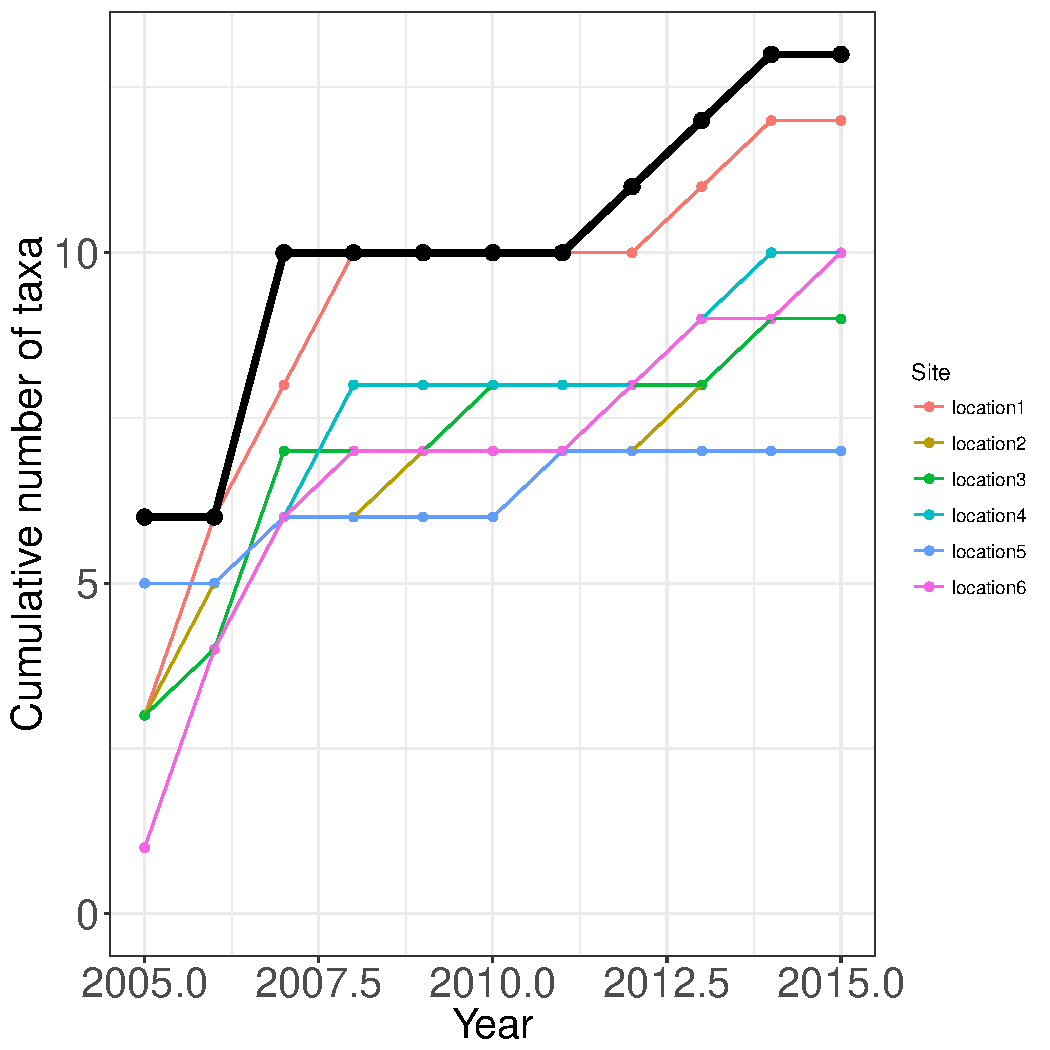
\includegraphics[scale = 0.4]{mcr-inverts-castorani_species_accumulation_curve.pdf}
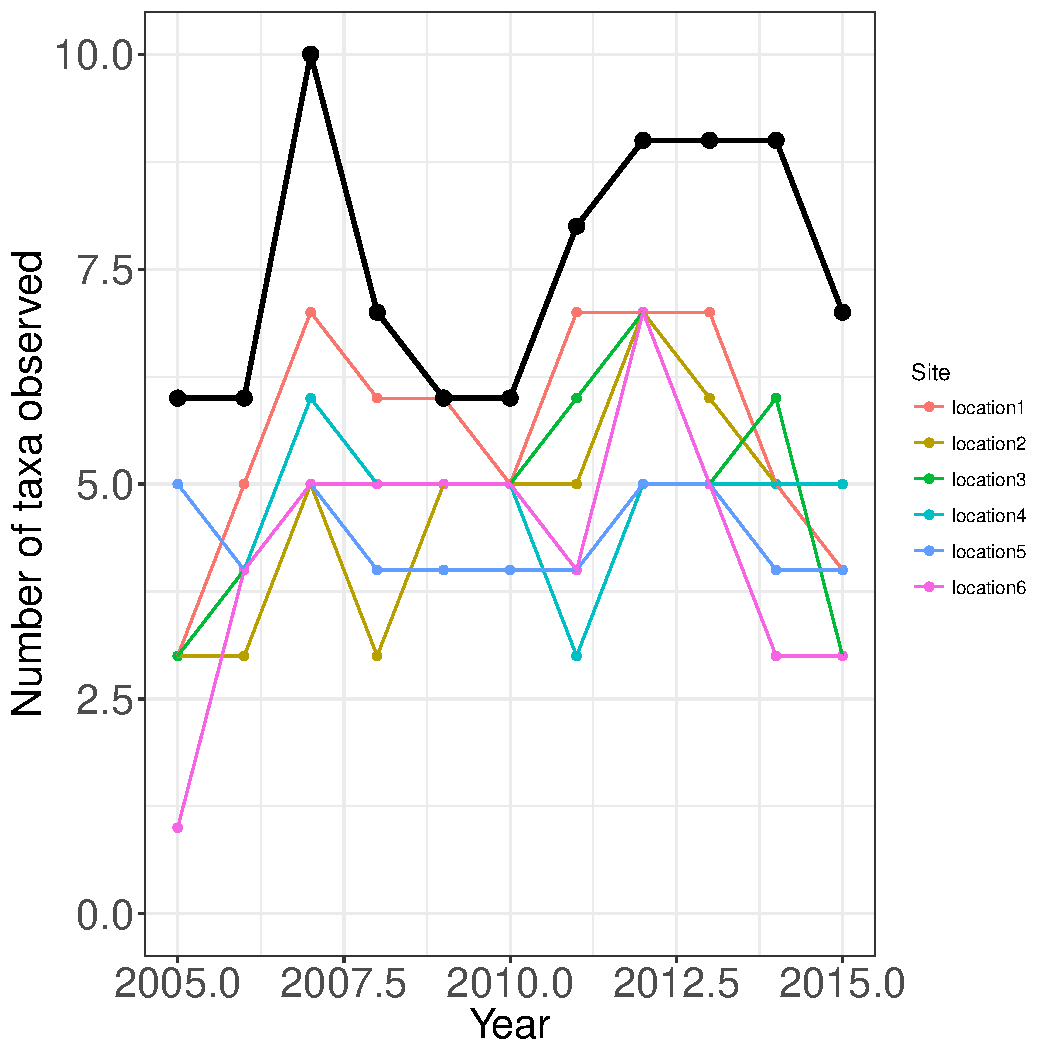
\includegraphics[scale = 0.4]{mcr-inverts-castorani_num_taxa_over_time.pdf}
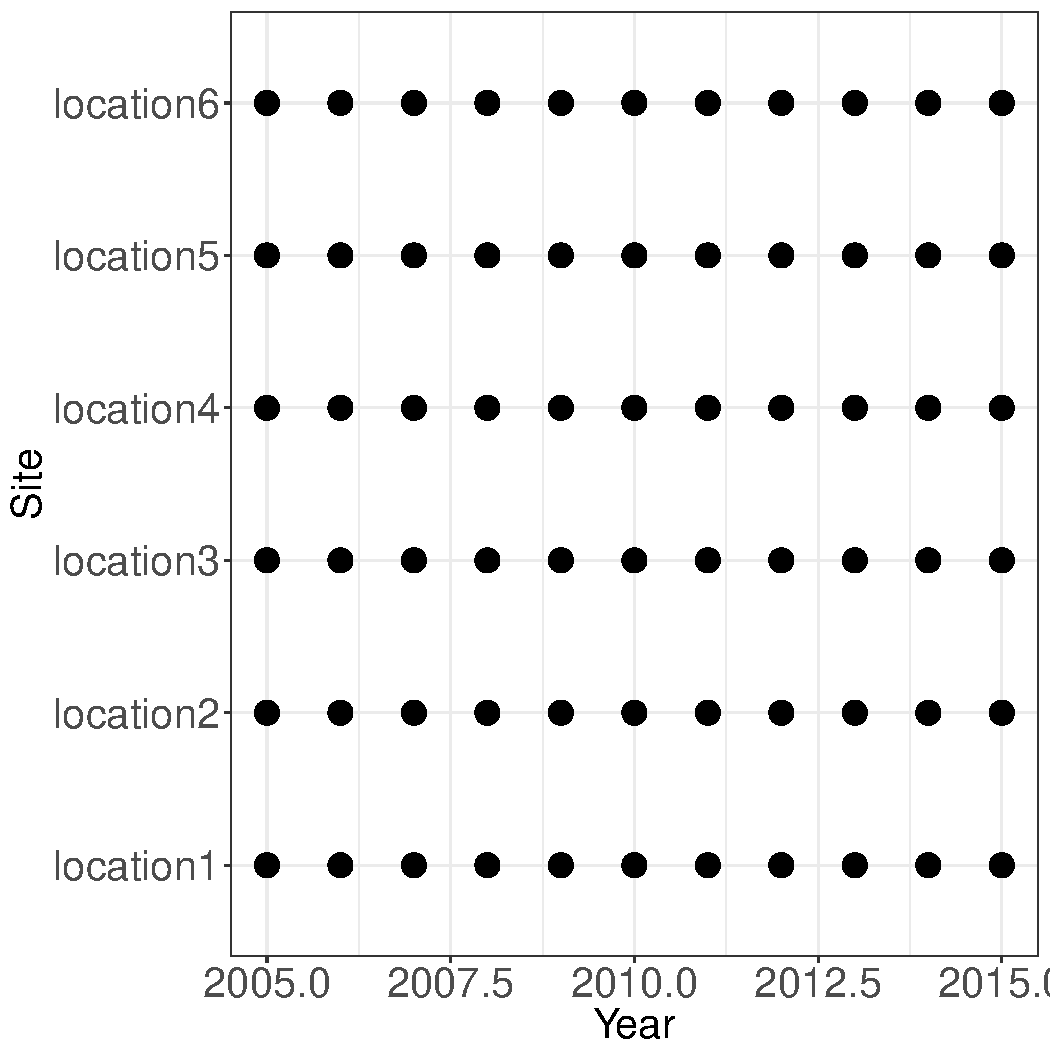
\includegraphics[scale = 0.4]{mcr-inverts-castorani_spatiotemporal_sampling_effort.pdf}
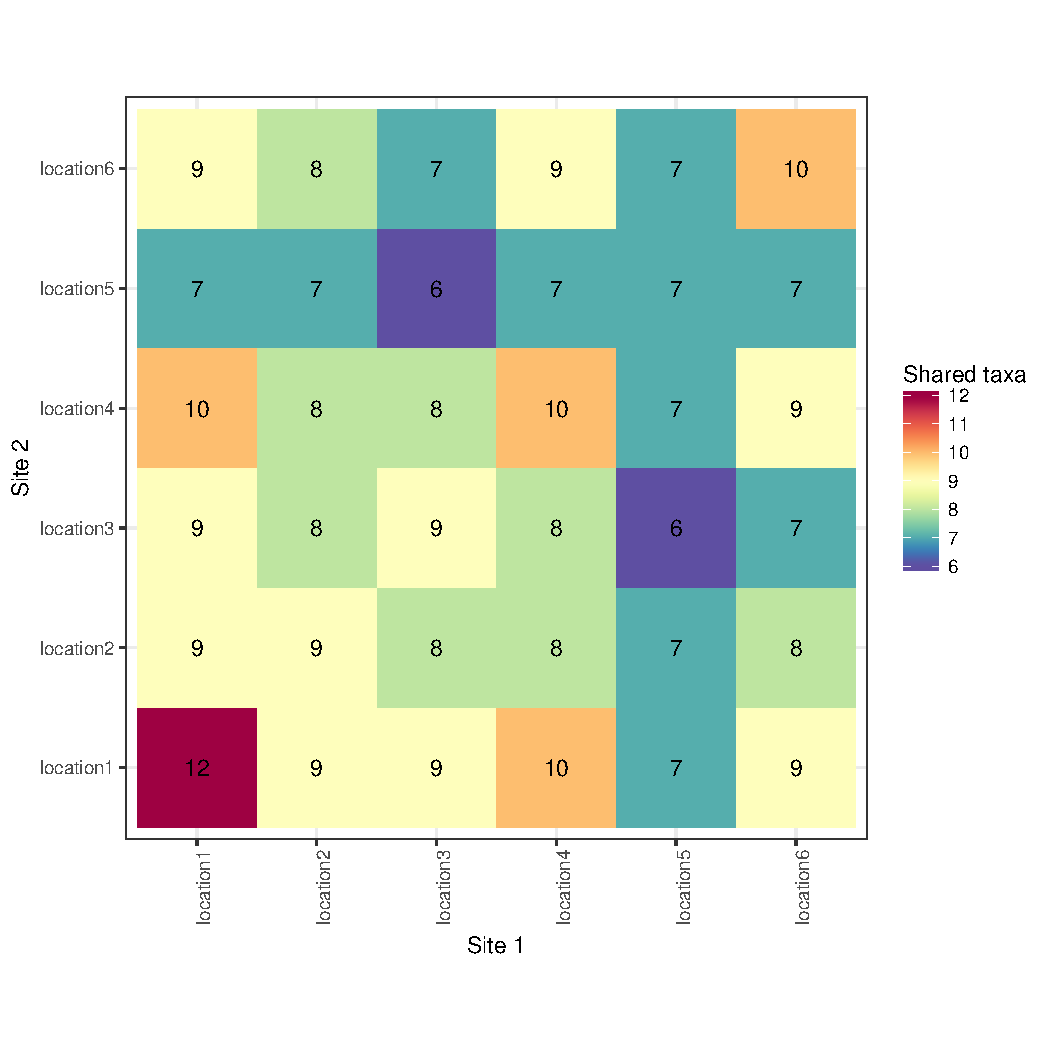
\includegraphics[scale = 0.4]{mcr-inverts-castorani_spp_shared.pdf}
\caption{{\bf MCR-inverts:} Species accumulation curves (top left),  annual richness (top right), and sampling effort (bottom)  for 13 invertebrate taxa observed at six sites on Moorea coral reef LTER (2006-2015). The black lines represent total site-level values across all plots.}
\label{mcr-inverts}
\end{figure}


\subsection {mcr-fish}
{\bf Updated data in ecocomdp format on EDI. Need to prepare it for this analysis. Need to separate by habitat. Needs data package citation.}
%Data were downloaded from EDI (knb-lter-mcr.6.54).
Data were aggregated across habitats and transects.
Thus each of the six sites contains data from very different habitats lumped together (backreef, forereef, fringing) and there is likely very little overlap in the species found in each habitat. 
This is different than the other datasets, and it would be good to discuss whether or not to separate by habitat.
Non-relevant taxa codes (e.g. ``No fish present") were removed from the dataset.
Abundance was recorded as dry biomass per 250 $m^2$, averaged across subplots, transects, and habitats for each species at each site in each year.
Data are in Figure \ref{mcr-fish}.
Six extra locations in forereef habitats were sampled in 2015.
These appear to be in addition to the four transects per habitat per site performed as part of the long term data collections, and thus they were removed from the dataset prior to analysis.
\begin{figure}[h!]
\centering
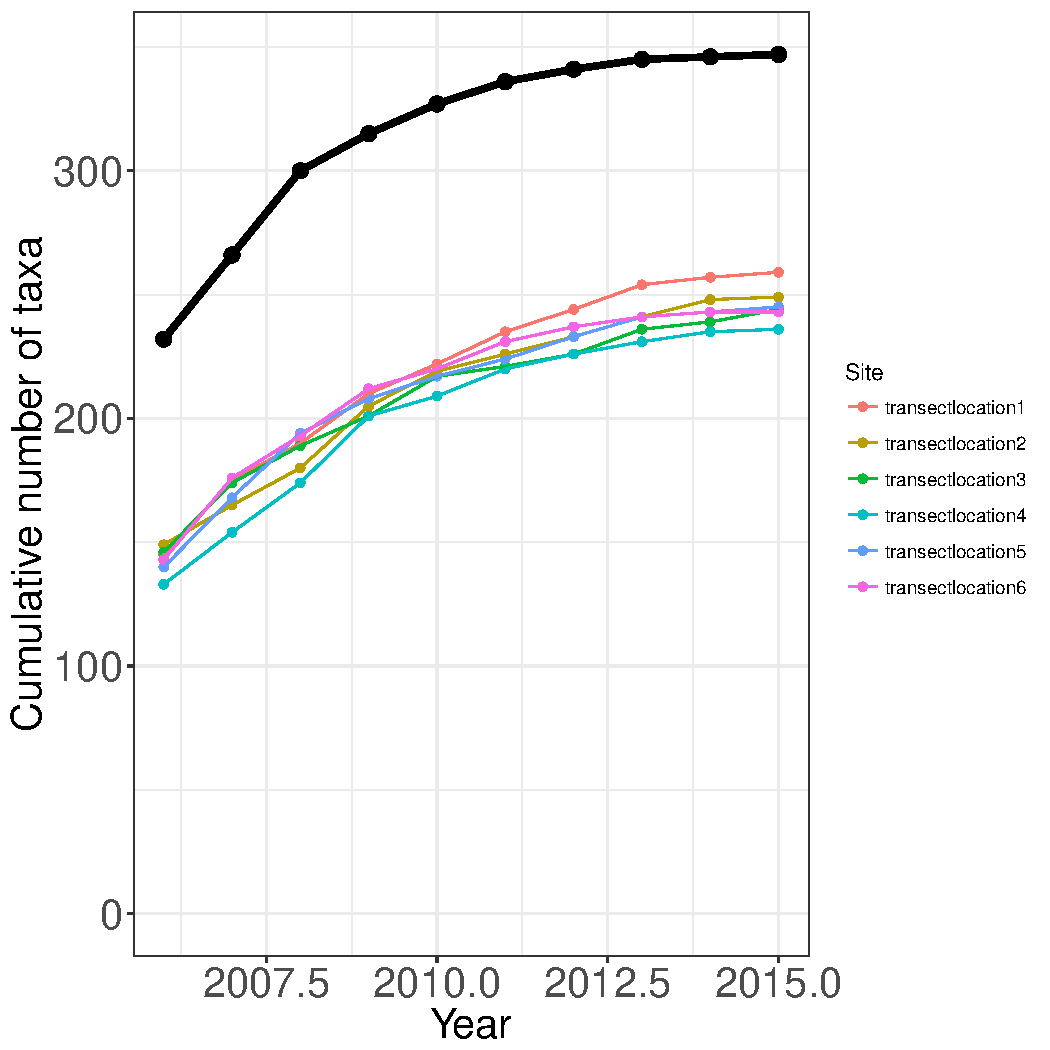
\includegraphics[scale = 0.4]{mcr-fish-castorani_species_accumulation_curve.pdf}
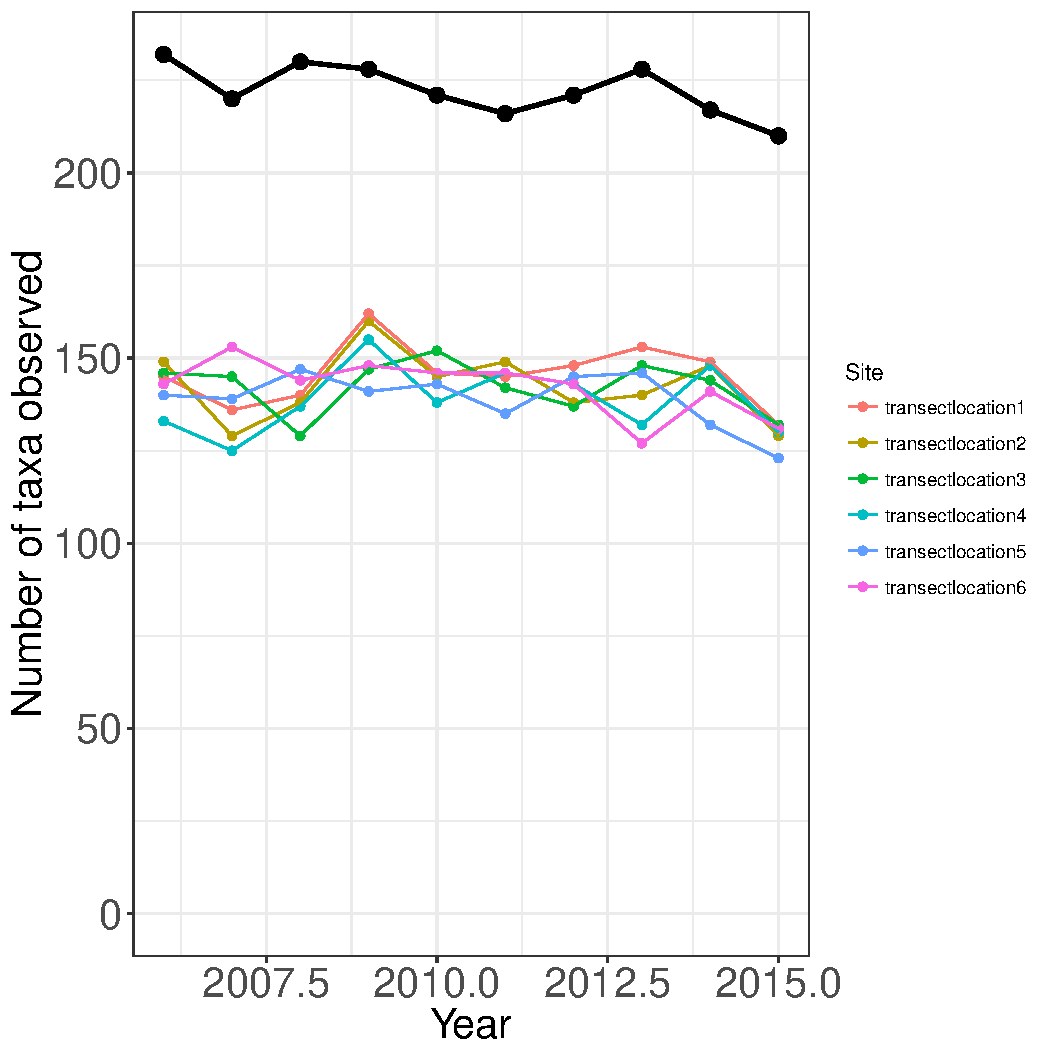
\includegraphics[scale = 0.4]{mcr-fish-castorani_num_taxa_over_time.pdf}
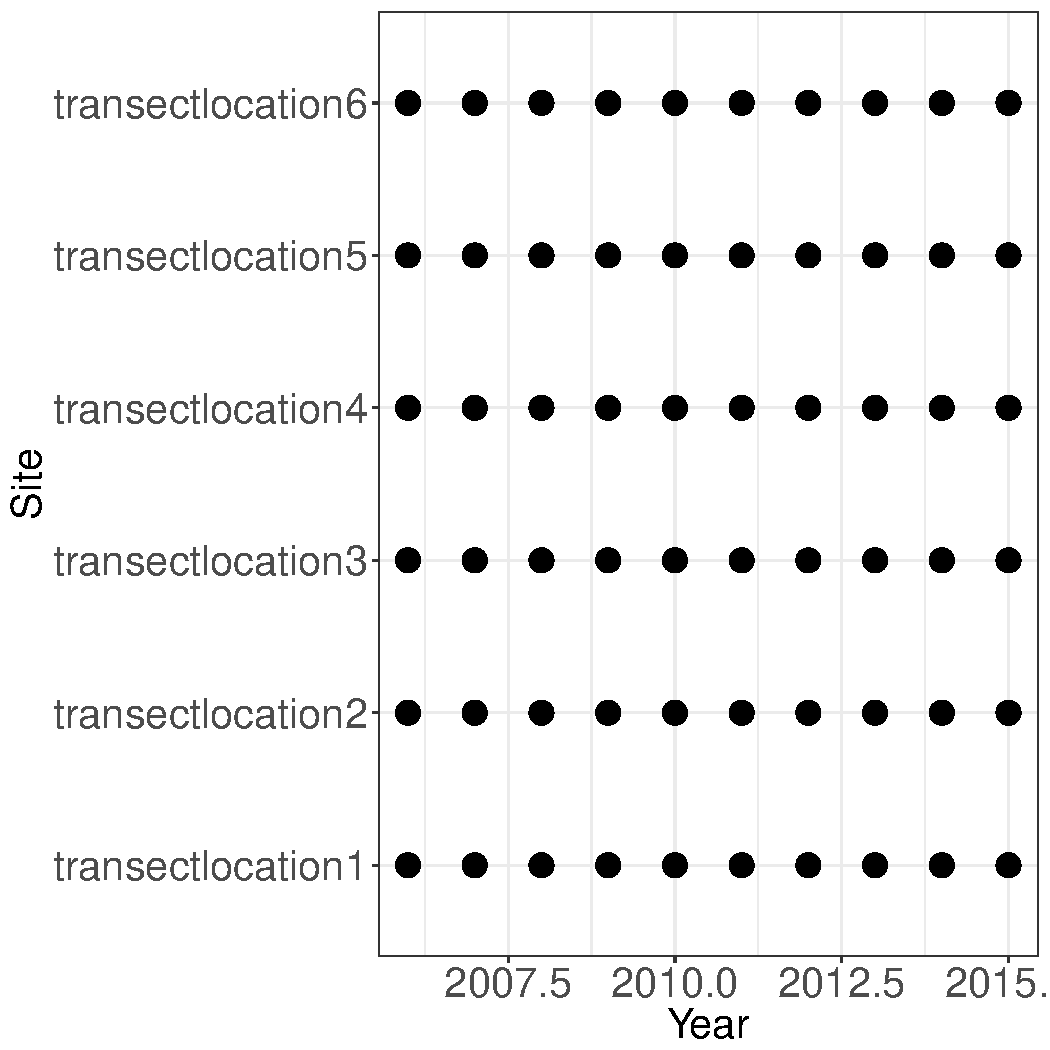
\includegraphics[scale = 0.4]{mcr-fish-castorani_spatiotemporal_sampling_effort.pdf}
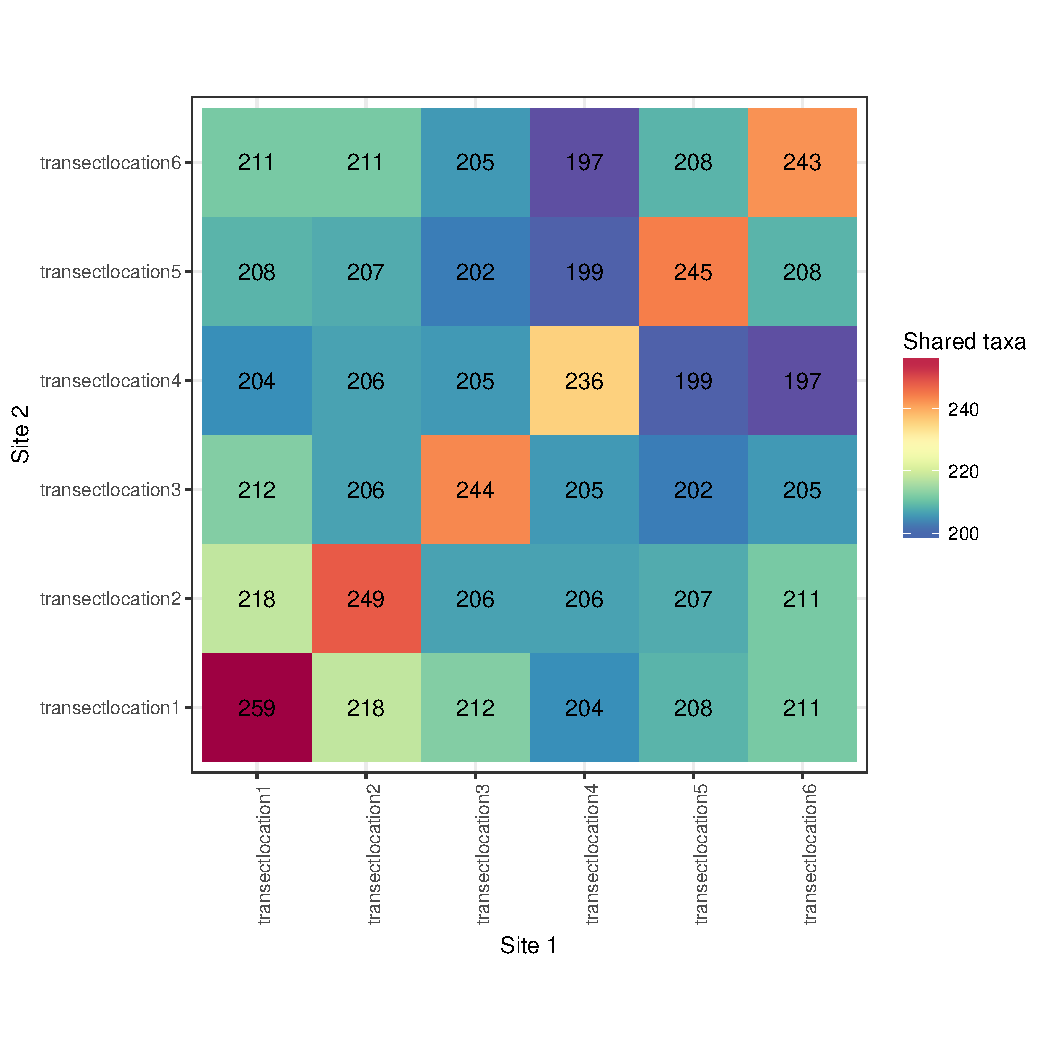
\includegraphics[scale = 0.4]{mcr-fish-castorani_spp_shared.pdf}
\caption{{\bf MCR-fish:} Species accumulation curves (top left),  annual richness (top right), and sampling effort (bottom)  for 377 fish taxa observed at six sites on Moorea coral reef LTER (2006-2015). The black lines represent total site-level values across all plots.}
\label{mcr-fish}
\end{figure}


\subsection {mcr-coral}
{\bf Need to get updated data. Need to separate by habitat. Needs data package citation.}
Data were downloaded from EDI \citep{mcr-coral}.
The corals are identified to the genus level.
Data were aggregated across habitats and transects.
Thus each of the six sites contains data from very different habitats lumped together (back, fringing, outer reefs) and there is likely very little overlap in the species found in each habitat. 
This is different than the other datasets, and it would be good to discuss whether or not to separate by habitat.
Non-relevant taxa were removed from the dataset.
Abundance was averaged across subplots, transects, and habitats for each species at each site in each year.
Data are in Figure \ref{mcr-coral}.
\begin{figure}[h!]
\centering
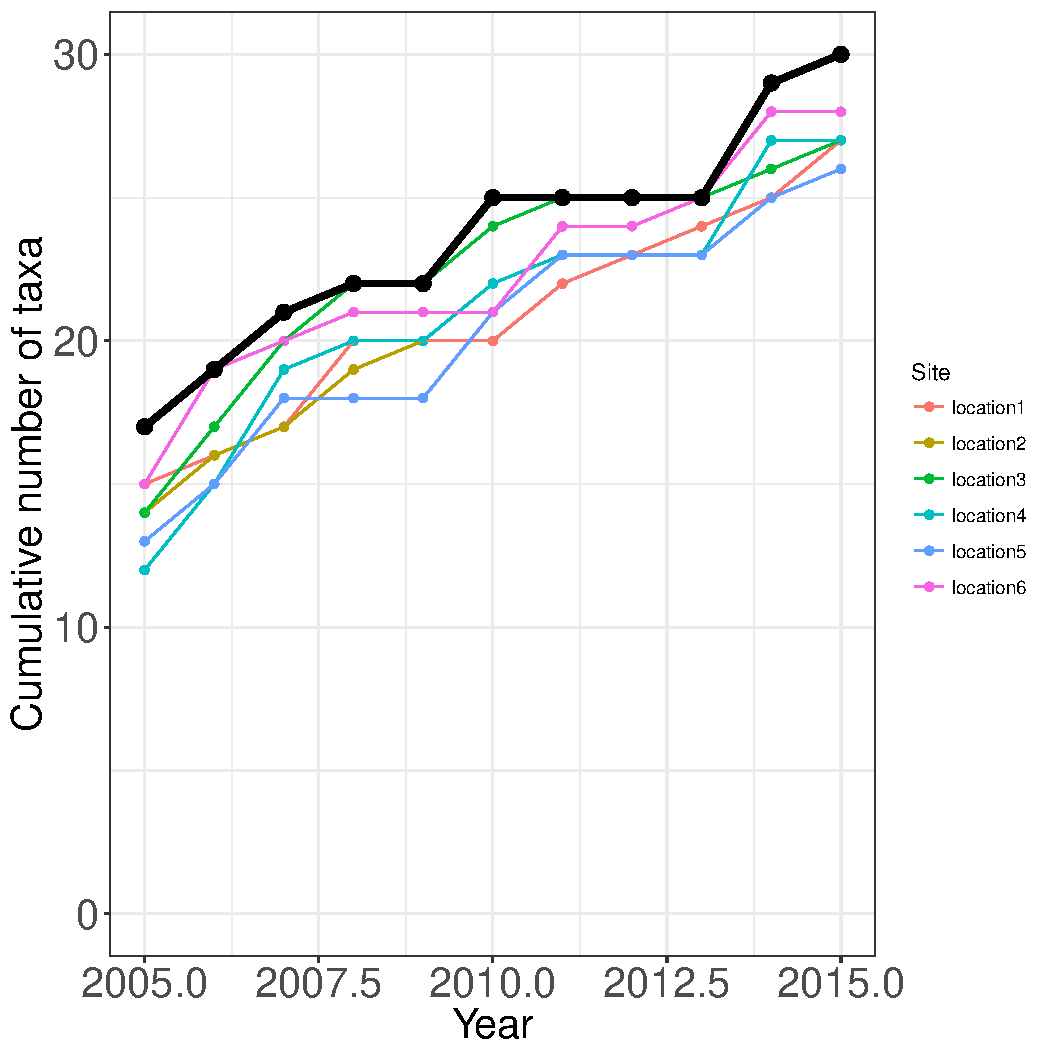
\includegraphics[scale = 0.4]{mcr-coral-castorani_species_accumulation_curve.pdf}
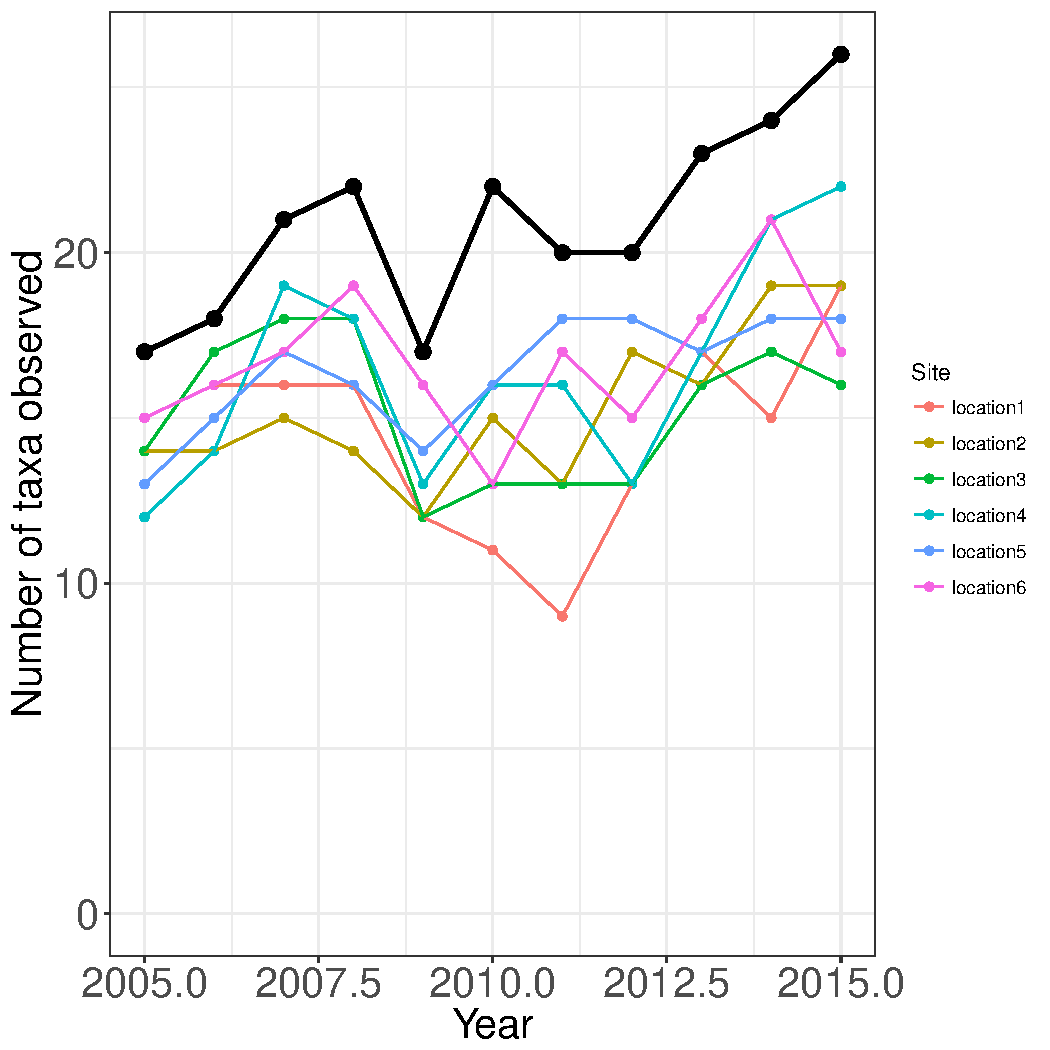
\includegraphics[scale = 0.4]{mcr-coral-castorani_num_taxa_over_time.pdf}
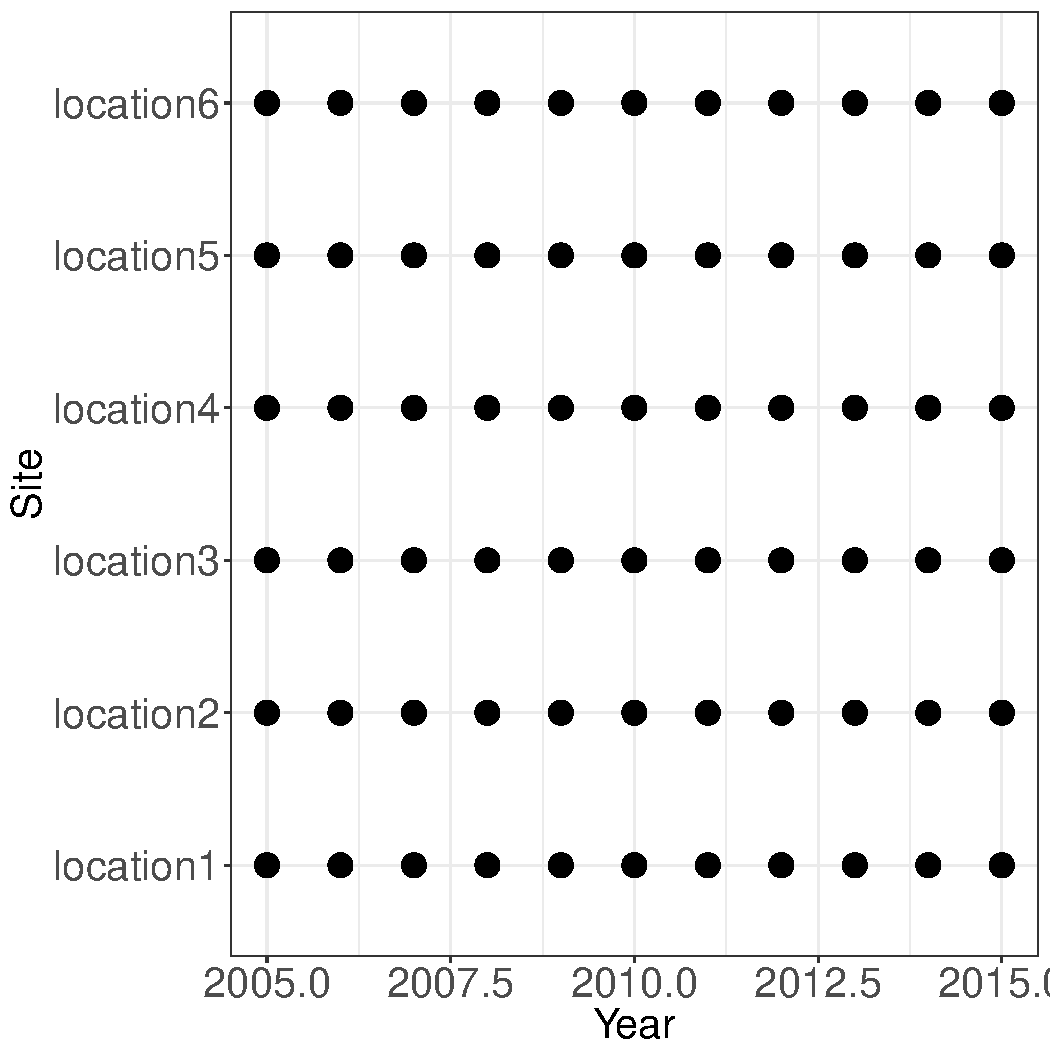
\includegraphics[scale = 0.4]{mcr-coral-castorani_spatiotemporal_sampling_effort.pdf}
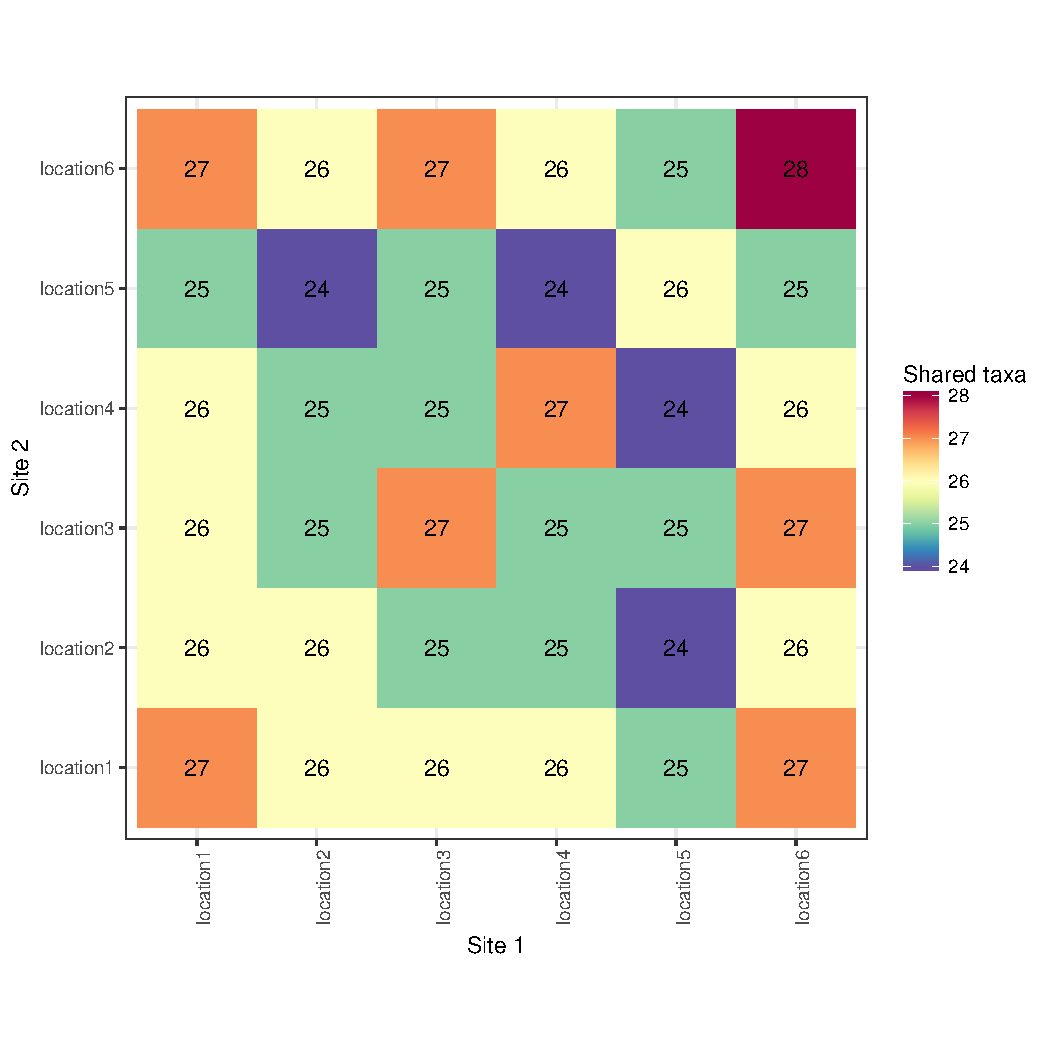
\includegraphics[scale = 0.4]{mcr-coral-castorani_spp_shared.pdf}
\caption{{\bf MCR-coral:} Species accumulation curves (top left),  annual richness (top right), and sampling effort (bottom)  for 31 coral taxa observed at six sites on Moorea coral reef LTER (2006-2015). The black lines represent total site-level values across all plots.}
\label{mcr-coral}
\end{figure}




\subsection {mcr-algae}
{\bf Need to get updated data. Need to separate by habitat. Needs data package citation.}
Data were downloaded from EDI \citep{mcr-algae}.
Data were aggregated across habitats and transects.
Thus each of the six sites contains data from very different habitats lumped together (back, fringing, outer reefs) and there is likely very little overlap in the species found in each habitat. 
This is different than the other datasets, and it would be good to discuss whether or not to separate by habitat.
Non-relevant taxa were removed from the dataset.
Abundance was averaged across subplots, transects, and habitats for each species at each site in each year.
Data are in Figure \ref{mcr-algae}.
The cumulative number of taxa was still increasing at the end of the time series.
\begin{figure}[h!]
\centering
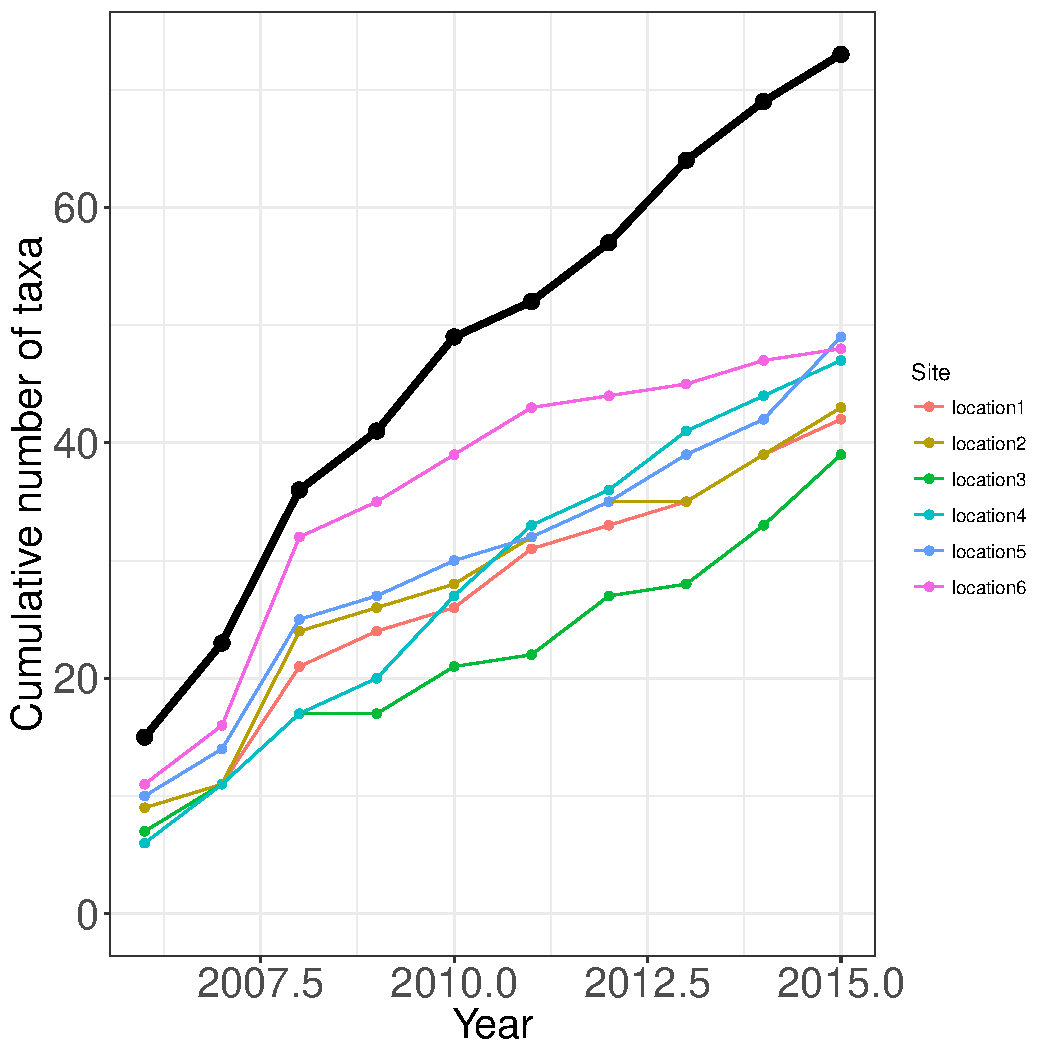
\includegraphics[scale = 0.4]{mcr-algae-castorani_species_accumulation_curve.pdf}
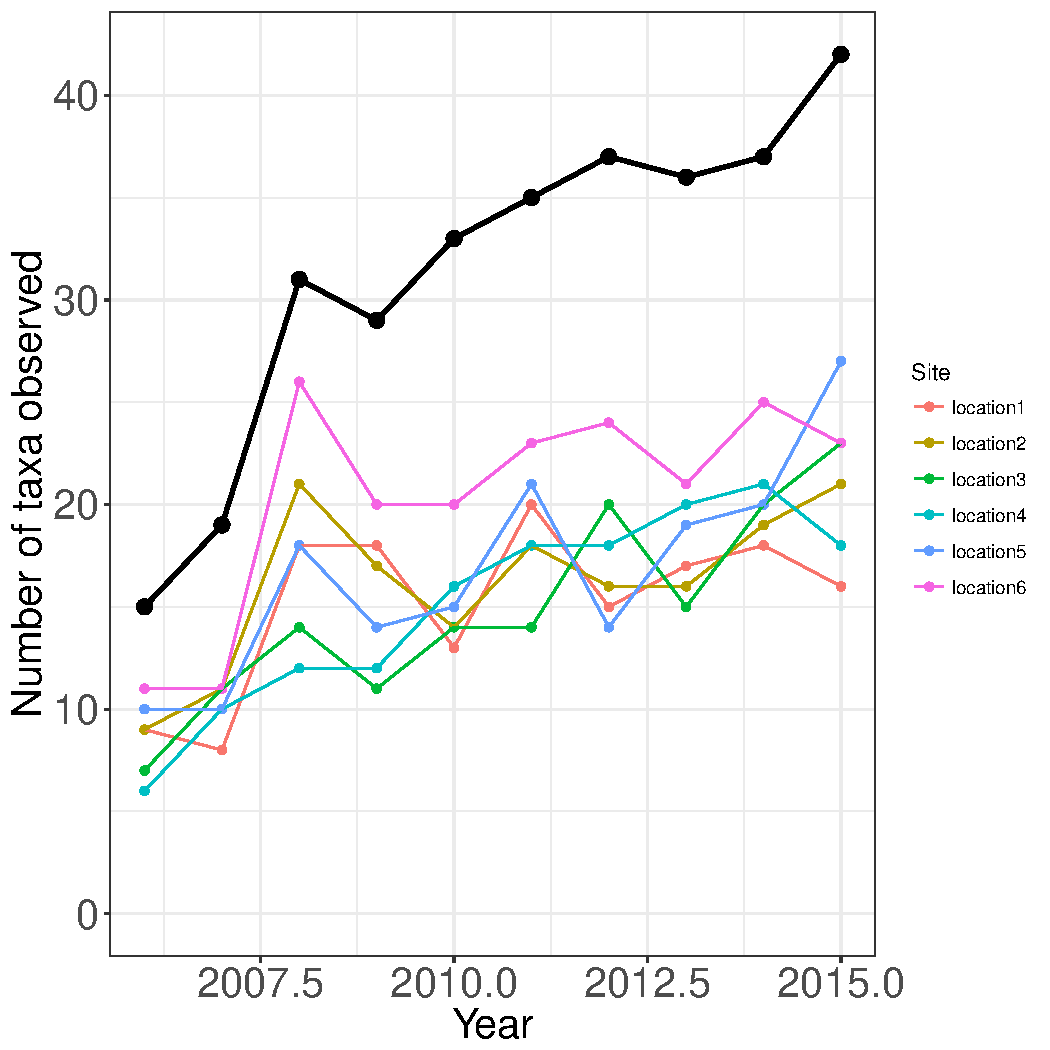
\includegraphics[scale = 0.4]{mcr-algae-castorani_num_taxa_over_time.pdf}
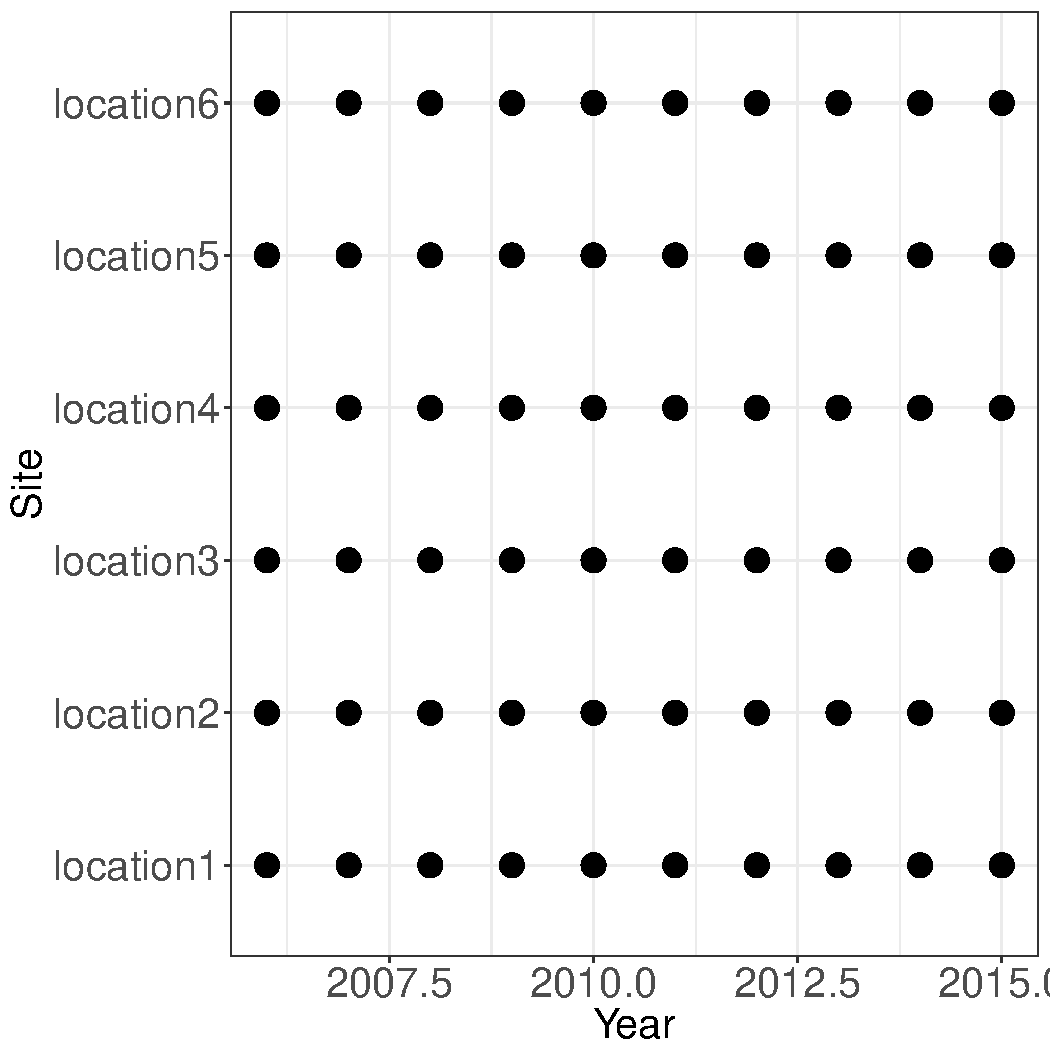
\includegraphics[scale = 0.4]{mcr-algae-castorani_spatiotemporal_sampling_effort.pdf}
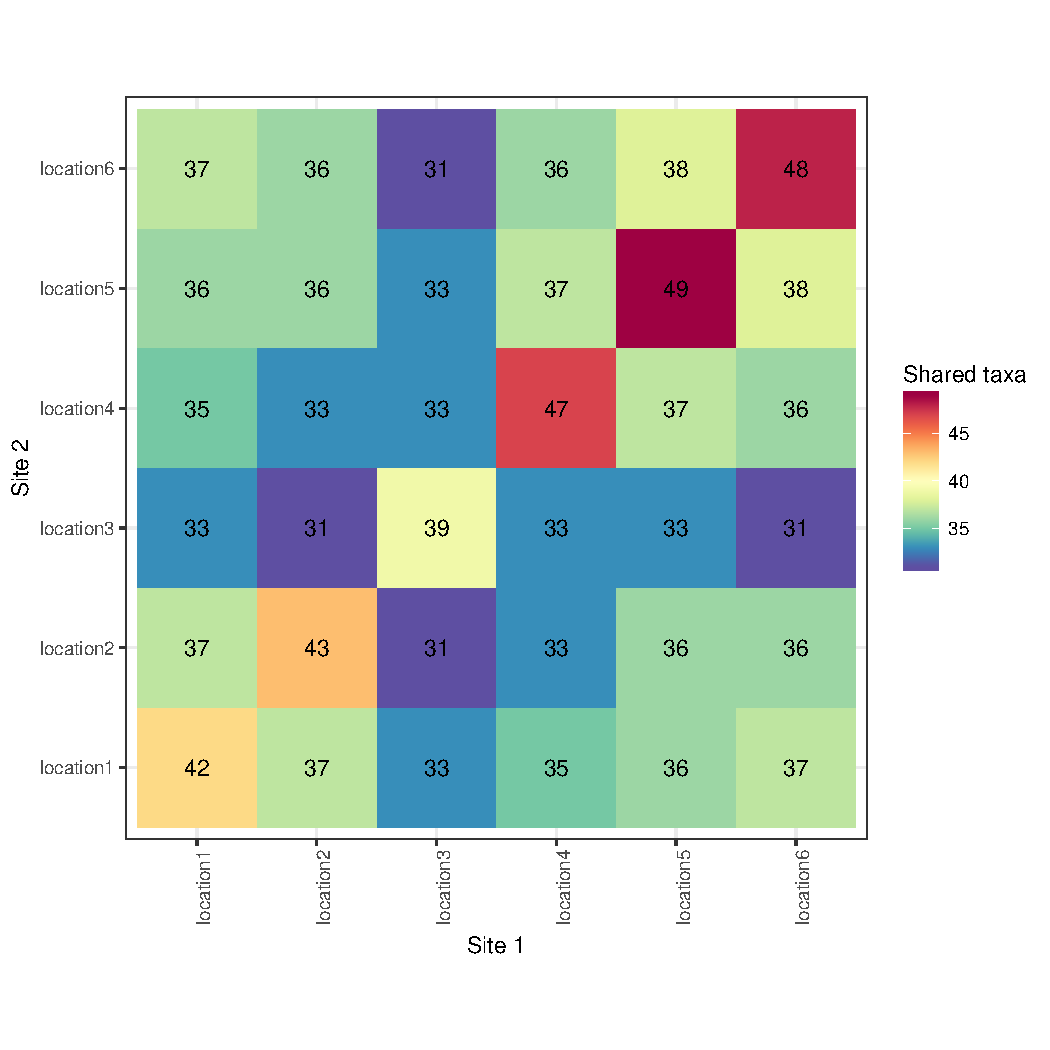
\includegraphics[scale = 0.4]{mcr-algae-castorani_spp_shared.pdf}
\caption{{\bf MCR-algae:} Species accumulation curves (top left),  annual richness (top right), and sampling effort (bottom)  for 73 algae taxa observed at six sites on Moorea coral reef LTER (2006-2015). The black lines represent total site-level values across all plots.}
\label{mcr-algae}
\end{figure}

%\subsection {mcm-diatoms}
%Each site was sampled anywhere from five to nine times over a 20 year period, but not all sites were sampled in all years.
%Data are in Figure \ref{mcm-diatoms}.
%We decided not to use this dataset.
%\begin{figure}[h!]
%\centering
%\includegraphics[scale = 0.4]{mcm-diatoms-schulteSokol_species_accumulation_curve.pdf}
%\includegraphics[scale = 0.4]{mcm-diatoms-schulteSokol_num_taxa_over_time.pdf}
%\includegraphics[scale = 0.4]{mcm-diatoms-schulteSokol_spatiotemporal_sampling_effort.pdf}
%\caption{{\bf MCM-diatoms:} Species accumulation curves (top left),  annual richness (top right), and sampling effort (bottom)  for 58 diatom taxa observed at five sites in McMurdo LTER.  The black lines represent total site-level values across all plots.}
%\label{mcm-diatoms}
%\end{figure}


%%%%%%%%%%%%%%%%%%%%%%
\section {Freshwater datasets}

\subsection {fce-diatoms}
{\bf Need to document where the data came from and clean the data.}
%Data are shown in Figure \ref{fce-diatoms}
There are over 171 sites in this dataset, but only a fraction of those were sampled in all seven years.
This could  contribute to variation in total number of taxa observed - the earlier years have the most missing sites and also the lowest total number of taxa.
Since the time series is so short to begin with, I suggest only including sites will all seven years in the analysis.
%\begin{figure}[h!]
%\centering
%\includegraphics[scale = 0.4]{fce-diatoms-marazzi_species_accumulation_curve.pdf}
%\includegraphics[scale = 0.4]{fce-diatoms-marazzi_num_taxa_over_time.pdf}
%\includegraphics[scale = 0.4]{fce-diatoms-marazzi_spatiotemporal_sampling_effort.pdf}
%\caption{{\bf FCE-diatoms:} Species accumulation curves (top left),  annual richness (top right), and sampling effort (bottom)  for 367 diatom taxa observed at 171 sites on Florida Coastal Everglades LTER. The black lines represent total site-level values across all plots.}
%\label{fce-diatoms}
%\end{figure}

\subsection {fce-algae}
{\bf Need to document where the data came from and clean the data.}
{\bf There are duplicated records in the dataset - NOT ready for analysis.}
The duplicates cause the errors in the metadata table and the missing figures.
%Data are shown in Figure \ref{fce-algae}
There are over 150 sites in this dataset, but only a fraction of those were sampled in all seven years.
Also, about 1/3 of all sited were not sampled in 2009, and it seems systematic (the sites with higher numbers were not sampled).
Notice the dip in number of taxa observed in 2009.
Since the time series is so short to begin with, I suggest only including sites will all seven years in the analysis.
%\begin{figure}[h!]
%\centering
%\includegraphics[scale = 0.4]{fce-algae-marazzi_species_accumulation_curve.pdf}
%\includegraphics[scale = 0.4]{fce-algae-marazzi_num_taxa_over_time.pdf}
%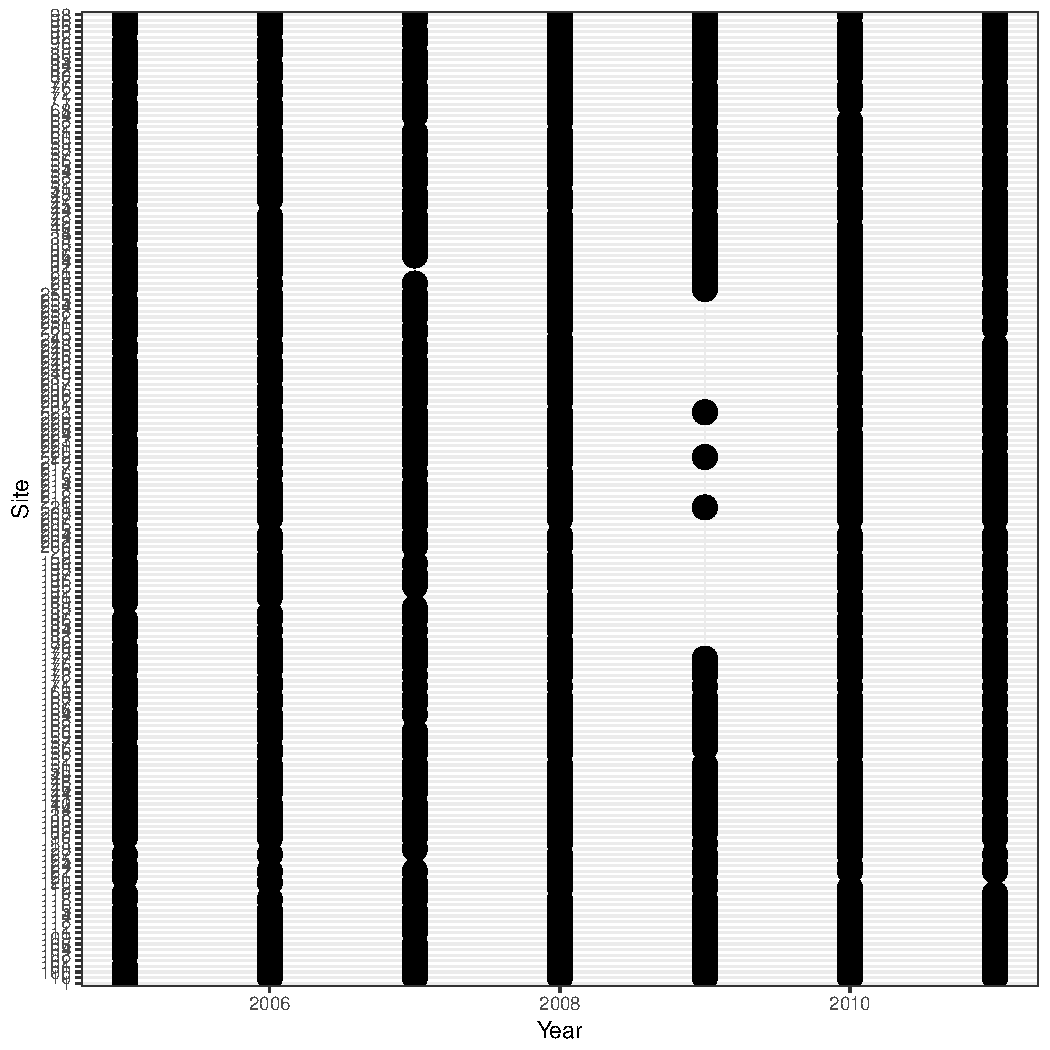
\includegraphics[scale = 0.4]{fce-algae-marazzi_spatiotemporal_sampling_effort.pdf}
%\caption{{\bf FCE-algae:} Species accumulation curves (top left),  annual richness (top right), and sampling effort (bottom)  for 249 algae taxa observed at lots of sites on Florida Coastal Everglades LTER. The black lines represent total site-level values across all plots.}
%\label{fce-algae}
%\end{figure}


\subsection {fce-fish}
Rolando obtained the data from the PI and is working on cleaning \citep{fce-fish}.
Data from the dry season are shown in Figure \ref{fce-fish-dry}.
Data from the wet season are shown in Figure \ref{fce-fish-wet}.

\begin{figure}[h!]
\centering
\includegraphics[scale = 0.4]{fce-fish-RehageDry_species_accumulation_curve.pdf}
\includegraphics[scale = 0.4]{fce-fish-RehageDry_num_taxa_over_time.pdf}
\includegraphics[scale = 0.4]{fce-fish-RehageDry_spatiotemporal_sampling_effort.pdf}
%\includegraphics[scale = 0.4]{fce-fish-RehageDry_spp_shared.pdf}
\caption{{\bf FCE-fish dry season:} Species accumulation curves (top left),  annual richness (top right), and sampling effort (bottom)  for fish taxa observed at the Florida Coastal Everglades . The black lines represent total site-level values across all plots.}
\label{fce-fish-dry}
\end{figure}

\begin{figure}[h!]
\centering
\includegraphics[scale = 0.4]{fce-fish-RehageWet_species_accumulation_curve.pdf}
\includegraphics[scale = 0.4]{fce-fish-RehageWet_num_taxa_over_time.pdf}
\includegraphics[scale = 0.4]{fce-fish-RehageWet_spatiotemporal_sampling_effort.pdf}
%\includegraphics[scale = 0.4]{fce-fish-RehageWet_spp_shared.pdf}
\caption{{\bf FCE-fish wet season:} Species accumulation curves (top left),  annual richness (top right), and sampling effort (bottom)  for fish taxa observed at the Florida Coastal Everglades . The black lines represent total site-level values across all plots.}
\label{fce-fish-wet}
\end{figure}



\newpage
\subsection {ntl-zooplankton}
The data were downloaded from the EDI Data Portal \citep{ntl-zooplankton}.
Samples were taken  via vertical tows at fortnightly intervals on a minimum of five occasions per year (range = 5 - 18 occasions per year).
Density was recorded as number of individuals per liter for each taxa, integrated volumetrically over the water column.
Many taxa are identified to species level, but some are identified to genus level.
Lake `Tr'  was only sampled in one year and was assumed to be the same as lake `TR'. %; thus we changed the lake identification code. 
The initial year (1981) was removed from analysis because only five of the seven lakes were sampled.
We additionally removed 165 records with missing or unknown taxa designations.
Data were aggregated annually for each taxa in each lake by taking the maximum density observed in a tow sampling occasion.
Data are shown in Figure \ref{ntl-zooplankton}.

\begin{figure}[h!]
\centering
\includegraphics[scale = 0.4]{ntl-zooplankton-stanleyLottig_species_accumulation_curve.pdf}
\includegraphics[scale = 0.4]{ntl-zooplankton-stanleyLottig_num_taxa_over_time.pdf}
\includegraphics[scale = 0.4]{ntl-zooplankton-stanleyLottig_spatiotemporal_sampling_effort.pdf}
\includegraphics[scale = 0.4]{ntl-zooplankton-stanleyLottig_spp_shared.pdf}
\caption{{\bf NTL-zooplankton:} Species accumulation curves (top left),  annual richness (top right), and sampling effort (bottom)  for 143 zooplankton taxa observed at 7 sites North Temperate Lakes LTER . The black lines represent total site-level values across all plots. The plot of the species accumulation curve failed because one site was sampled in only one year, and will be fixed once that site is removed.}
\label{ntl-zooplankton}
\end{figure}


%\subsection {ntl-macroinvertebrate}
%{\bf The data have not been propagated (i.e. no zero values recorded when a species is absent) and are NOT ready for analysis.}
%Data are shown in Figure \ref{ntl-macroinvertebrate}.
%There are only four taxa in this dataset (Chaoborus, Leptodora, Mysis, and Bythotrephes).
%I don't think that's enough species to meet our criteria.
%Also note that in some years there appear to be five taxa because Chaoborus larvae and Chaoborus pupae were given separate IDs. 
%This needs to be fixed prior to analysis.
%Also, it's unclear whether the data are not propagated, or not all taxa were counted in all years.
%Four of the 7 sites were not sampled in 1998.
%I think that year (1998) should be removed.
%But mostly, I don't think this dataset meets the criteria.
%\begin{figure}[h!]
%\centering
%\includegraphics[scale = 0.4]{ntl-macroinvertebrate-stanleyLottig_species_accumulation_curve.pdf}
%\includegraphics[scale = 0.4]{ntl-macroinvertebrate-stanleyLottig_num_taxa_over_time.pdf}
%\includegraphics[scale = 0.4]{ntl-macroinvertebrate-stanleyLottig_spatiotemporal_sampling_effort.pdf}
%\caption{{\bf NTL-macroinvertebrates:} Species accumulation curves (top left),  annual richness (top right), and sampling effort (bottom)  for 4 macroinvertabrate taxa observed at 7 sites North Temperate Lakes LTER . The black lines represent total site-level values across all plots.}
%\label{ntl-macroinvertebrate}
%\end{figure}


\subsection {ntl-fish}

Data on fish abundance were downloaded from the EDI Data Portal \citep{ntl-fish}.
Two types of gill nets (VGN and VGN127) and the method  ``ESHOCK" were rarely used, and thus removed from the dataset.% as per a conversation with Noah Lottig at NTL.
%The gear method ``ESHOCK" was also rarely used and a follow up call is needed to determine how best to handle those data.
%They are currently included.
Catch per unit effort (CPUE) was calculated for each species in each lake per year across all gear types (electrofishing, gill nets, baited traps) as the total catch divided by the total effort.
%We should double check with dataset contacts to be sure we did this correctly.
88 rows containing unidentified species were removed.
Also, the two bog lakes (CB, TB) had 1-3 species each and were removed. 
Three of the 11 sites (FI, MO, WI) were initiated in 1995, and therefore the time series was subsetted to include only years after 1994.
Data are shown in Figure \ref{ntl-fish}.


\begin{figure}[h!]
\centering
\includegraphics[scale = 0.4]{ntl-fish-stanleyLottig_species_accumulation_curve.pdf}
\includegraphics[scale = 0.4]{ntl-fish-stanleyLottig_num_taxa_over_time.pdf}
\includegraphics[scale = 0.4]{ntl-fish-stanleyLottig_spatiotemporal_sampling_effort.pdf}
\includegraphics[scale = 0.4]{ntl-fish-stanleyLottig_spp_shared.pdf}
\caption{{\bf NTL-fish:} Species accumulation curves (top left),  annual richness (top right), and sampling effort (bottom)  for 81 fish species observed at 9 lakes in the North Temperate Lakes LTER (1995-2016). The black lines represent total site-level values across all plots.}
\label{ntl-fish}
\end{figure}


%%%%%%%%%%%%%%%%%%%
\section {Terrestrial datasets}

\subsection {nwt-plants}
{\bf no provenance.}
The data were obtained from Eric Sokol.
Not all years were sampled, but all plots were sampled in each year of observation. 
 Number of taxa increased rapidly toward the end of the time series. 
 Data in Figure \ref{nwt-plants}.
 It would be good to collect more metadata and provenance for this dataset.
 The plots comprise at least four distinct habitats.
 Some plots have very few species.

\begin{figure}[h!]
\centering
\includegraphics[scale = 0.4]{nwt-plants-hallett_species_accumulation_curve.pdf}
\includegraphics[scale = 0.4]{nwt-plants-hallett_num_taxa_over_time.pdf}
\includegraphics[scale = 0.4]{nwt-plants-hallett_spatiotemporal_sampling_effort.pdf}
\includegraphics[scale = 0.4]{nwt-plants-hallett_spp_shared.pdf}
\caption{{\bf NWT-plants:} Species accumulation curves (top left),  annual richness (top right), and sampling effort (bottom)  for 109 plant species observed at 88 plots in the Niwot Ridge LTER (1989-2014). The black lines represent total site-level values across all plots.}
\label{nwt-plants}
\end{figure}


\subsection {and-plants-mtStHelens}
Data were downloaded from Ecologcial Archives \citep{and-plants}.
here it is (Figure \ref{and-plants}).

\begin{figure}[h!]
\centering
\includegraphics[scale = 0.4]{and-plants-mtStHelens_species_accumulation_curve.pdf}
\includegraphics[scale = 0.4]{and-plants-mtStHelens_num_taxa_over_time.pdf}
\includegraphics[scale = 0.4]{and-plants-mtStHelens_spatiotemporal_sampling_effort.pdf}
\includegraphics[scale = 0.4]{and-plants-mtStHelens_spp_shared.pdf}
\caption{{\bf AND-plants:} Species accumulation curves (top left),  annual richness (top right), and sampling effort (bottom)  for plant species observed at Mt. St. Helens. The black lines represent total site-level values across all plots.}
\label{and-plants}
\end{figure}


\subsection {cdr-plants}
Data were downloaded from EDI \citep{cdr-plants}.
Needs cleaning still (Figure \ref{cdr-plants}).

\begin{figure}[h!]
\centering
\includegraphics[scale = 0.4]{cdr-plants-compagnoni_species_accumulation_curve.pdf}
\includegraphics[scale = 0.4]{cdr-plants-compagnoni_num_taxa_over_time.pdf}
\includegraphics[scale = 0.4]{cdr-plants-compagnoni_spatiotemporal_sampling_effort.pdf}
\includegraphics[scale = 0.4]{cdr-plants-compagnoni_spp_shared.pdf}
\caption{{\bf CDR-plants:} Species accumulation curves (top left),  annual richness (top right), and sampling effort (bottom)  for plant species observed at Cedar Creek. The black lines represent total site-level values across all plots.}
\label{cdr-plants}
\end{figure}



\subsection {jrn-lizards}
The data were downloaded from the EDI Data Portal \citep{jrn-lizard}.
This was a mark-recapture study. 
Pitfall traps were opened for two weeks four times per year (quarterly). 
The monthly samples from 1990 and 1991 were removed.
Individual lizards were identified and the number of unique individuals per site per year were summed. 
Two sites that were established five years after the start of the study (SUMM and NORT) were excluded. 
We don't have a key to the species codes.
Data are shown in Figure \ref{jrn-lizards}.
The cumulative number of taxa was still increasing at the end of the time series, although with only 20 species total one or two species introductions could cause this pattern.


\begin{figure}[h!]
\centering
\includegraphics[scale = 0.4]{jrn-lizards-hope_species_accumulation_curve.pdf}
\includegraphics[scale = 0.4]{jrn-lizards-hope_num_taxa_over_time.pdf}
\includegraphics[scale = 0.4]{jrn-lizards-hope_spatiotemporal_sampling_effort.pdf}
\includegraphics[scale = 0.4]{jrn-lizards-hope_spp_shared.pdf}
\caption{{\bf JRN-lizards:} Species accumulation curves (top left),  annual richness (top right), and sampling effort (bottom)  for 20 lizard species observed at 9 plots in the Jornada LTER (1990-2005). The black lines represent total site-level values across all plots.}
\label{jrn-lizards}
\end{figure}



\subsection {cap-herps}
The data were downloaded from the EDI Data Portal \citep{cap-herps}.
Data are shown in Figure \ref{cap-herps}.
This is a visual encounter survey where herpetofauna observations were nested by 3 plots within 3 transects per site. 
Each site represents the reach level (each reach level site is composed of 3 transects with equal area sampling efforts). 
Surveys from 2012 and March were dropped to standardize sampling efforts temporally. 
Unidentified species were dropped, species code is the scientific name of species. 
Taxon count was calculated as the maximum abundance per year in any one of the sampling events (with 3 sampling events per reach in April/May, June/July, and September/October). 
%The final community dataset prepared for analysis has 7 sites representative of the reach level metacommunity dynamics (3 transects sampled per reach) from 2013-2017 with a total of 18 observed species across all sites.  

\begin{figure}[h!]
\centering
\includegraphics[scale = 0.4]{cap-herps-banville_species_accumulation_curve.pdf}
\includegraphics[scale = 0.4]{cap-herps-banville_num_taxa_over_time.pdf}
\includegraphics[scale = 0.4]{cap-herps-banville_spatiotemporal_sampling_effort.pdf}
\includegraphics[scale = 0.4]{cap-herps-banville_spp_shared.pdf}
\caption{{\bf CAP-herps:} Species accumulation curves (top left),  annual richness (top right), and sampling effort (bottom)  for species observed in the Central Area Phoenix LTER (1990-2005). The black lines represent total site-level values across all plots.}
\label{cap-herps}
\end{figure}



\subsection {sev-grasshoppers}
The data were downloaded from the EDI Data Portal \citep{sev-grasshopper}.
Data are shown in Figure \ref{sev-grasshoppers}.
  

\begin{figure}[h!]
\centering
\includegraphics[scale = 0.4]{sev-grasshopper-compagnoni_species_accumulation_curve.pdf}
\includegraphics[scale = 0.4]{sev-grasshopper-compagnoni_num_taxa_over_time.pdf}
\includegraphics[scale = 0.4]{sev-grasshopper-compagnoni_spatiotemporal_sampling_effort.pdf}
\includegraphics[scale = 0.4]{sev-grasshopper-compagnoni_spp_shared.pdf}
\caption{{\bf SEV-grasshoppers:} Species accumulation curves (top left),  annual richness (top right), and sampling effort (bottom)  for grasshopper species observed in the Sevilleta LTER. The black lines represent total site-level values across all plots.}
\label{sev-grasshoppers}
\end{figure}


\subsection {and-birds}
The data were downloaded from the EDI Data Portal \citep{and-birds}.
Data are shown in Figure \ref{and-birds}.

\begin{figure}[h!]
\centering
\includegraphics[scale = 0.4]{and-birds-wisnoski_species_accumulation_curve.pdf}
\includegraphics[scale = 0.4]{and-birds-wisnoski_num_taxa_over_time.pdf}
\includegraphics[scale = 0.4]{and-birds-wisnoski_spatiotemporal_sampling_effort.pdf}
%\includegraphics[scale = 0.4]{and-birds-wisnoski_spp_shared.pdf}
\caption{{\bf AND-birds:} }
\label{and-birds}
\end{figure}


\subsection {hbr-birds}
{\bf Need to subset by date so only 1-2 sampling occasions per year are included.}
These point count data were downloaded from the EDI Data Portal \citep{hbr-birds}.
Years with highly incomplete sampling were removed (1999, 2000, 2008) and only plots that were sampled in all of the remaining years were retained for analysis.
The number of individuals of each species within 50 m of the `point' was summed for each 10-minute plot visit, using the `NewRecord' column to identify unique individuals for data collected after 2005. 
The maximum number of individuals of each species for each plot-year (across 1-3 sampling occasions in June/early July per year)  was calculated.
Data are shown in Figure \ref{hbr-birds}.


\begin{figure}[h!]
\centering
\includegraphics[scale = 0.4]{hbr-birds-sillett_species_accumulation_curve.pdf}
\includegraphics[scale = 0.4]{hbr-birds-sillett_num_taxa_over_time.pdf}
\includegraphics[scale = 0.4]{hbr-birds-sillett_spatiotemporal_sampling_effort.pdf}
\includegraphics[scale = 0.4]{hbr-birds-sillett_spp_shared.pdf}
\caption{{\bf HBR-birds:} }
\label{hbr-birds}
\end{figure}

\subsection{cap-birds}
Data were obtained from EDI \citep{cap-birds}.
Data are shown in Figure \ref{cap-birds}.
This is a point count study where birds were observed (seen or heard) for 15 minutes within a 40 m fixed radius. 
Each site represents one point count. 
Only ESCA point counts are included. 
Data from 2017 were dropped because not all sites were sampled. 
Four point count sites (M-9, V-18, X-8, and V-16) were dropped due to uneven sampling across years. 
Unidentified species accounted for less then 2\% of the total data and were dropped. 
%Species codes are 4-letter codes (https://www.wintuaudubon.org/Documents/Alpha_codes_eng.pdf). 
Taxon count was calculated as the maximum abundance per year during the spring month's sampling events (with 3 sampling events per site between March, April, and May). 
  

\begin{figure}[h!]
\centering
\includegraphics[scale = 0.4]{cap-birds-banville_species_accumulation_curve.pdf}
\includegraphics[scale = 0.4]{cap-birds-banville_num_taxa_over_time.pdf}
\includegraphics[scale = 0.4]{cap-birds-banville_spatiotemporal_sampling_effort.pdf}
\includegraphics[scale = 0.4]{cap-birds-banville_spp_shared.pdf}
\caption{{\bf CAP-birds:} }
\label{cap-birds}
\end{figure}




\bibliographystyle{apalike}
\renewcommand{\refname}{\subsection*{References}}
\bibliography{LTER_metacom}

\end{document}